\documentclass{article}
\usepackage[T1]{fontenc}
\usepackage[utf8]{inputenc}
\usepackage[italian]{babel}
\usepackage{graphicx}
\usepackage{amsmath,amssymb}
\usepackage{listings}
\usepackage{color}
\definecolor{mygreen}{RGB}{28,172,0} % color values Red, Green, Blue
\definecolor{mylilas}{RGB}{170,55,241}
\usepackage[a4paper,top=2cm,bottom=2cm,left=2cm,right=2cm]{geometry}
\lstset{language=Matlab,%
    %basicstyle=\color{red},
    breaklines=true,%
    morekeywords={matlab2tikz},
    keywordstyle=\color{blue},%
    morekeywords=[2]{1}, keywordstyle=[2]{\color{black}},
    identifierstyle=\color{black},%
    stringstyle=\color{mylilas},
    commentstyle=\color{mygreen},%
    showstringspaces=false,%without this there will be a symbol in the places where there is a space
    numbers=left,%
    numberstyle={\tiny \color{black}},% size of the numbers
    numbersep=9pt, % this defines how far the numbers are from the text
    emph=[1]{for,end,break},emphstyle=[1]\color{red}, %some words to emphasise
    %emph=[2]{word1,word2}, emphstyle=[2]{style},    
}

\newcommand{\vs}{\vspace*{1.0cm}}
\graphicspath{ {images/} }

\begin{document}
  \author{Lorenzo Pattarini}
  \title{Relazioni di Calcolo Numerico}
  \maketitle
 

  \tableofcontents


%%%%%%%%%%%%%%%%%%%%%%%%%%%%%%%%%%%%%%%%%%%%%%%%%%%%%%%%%%%%%%%%%%%%%%%%%%%%%%%%%%%%%
%%%%%%%%%%%%%%%%%%%%%%%%%%%%%%%%%%%%%%%%%%%%%%%%%%%%%%%%%%%%%%%%%%%%%%%%%%%%%%%%%%%%%

\newpage
\section{ Esercitazione 1}


%%%%%%%%%%%%%%%%%%%%%%%%%%%%%%%%%%%%%%%%%%%%%%%%%%%%%%%%%%%%%%%%%%%%%%%%%%%%%%%%%%%%%

\subsection{ Esercizio 1}
\begin{lstlisting}
a = 1.12;
b = 2.34;
c = 0.72;
d = 0.81;
e = 3;
f = 19.83;
g = 20;

x = 1+a/b+c/(f^2);
s = (b-a)/(d-c);
z = (1-(1/(e^5)))^(-1);
r = 1/(1/a+1/c+1/c+1/d);
y = a*b*(1/c)*(f^2/2);
t = 7*(g^(1/3))+4*g^(0.58);

format short
x s z r y t

format long
x s z r y t

\end{lstlisting}


%%%%%%%%%%%%%%%%%%%%%%%%%%%%%%%%%%%%%%%%%%%%%%%%%%%%%%%%%%%%%%%%%%%%%%%%%%%%%%%%%%%%%
\vs
\subsection{ Esercizio 2}
\begin{lstlisting}
% Ricerca degli errori sintattici

a = 2y+(((3+1)9);

  % Manca una parentesi e la variabile y non risulta inizializzata

b == 2*sin[3];

  %{
     L'operatore "==" \'{e} un operatore di testing non di 
     assegnamento, ma non essendo la variabile b inizializzata
     non ha senso testarne l'uguaglianza.
     Il secondo errore \'{e} l'ultilizzo delle parentesi quadre in quanto, 
     per riferirsi all'argomento di una funzione vanno usate le
     parentesi tonde.
  %} 

c = e^0.5;

  %{
     Il modo corretto per ottenere la radice del numero di nepero
     \'{e} c = exp(0.5).
  %}

d = log(4-8/4*2)

  %{
     In questo modo non essendo certi della precedenza degli operatori
     rischiamo di tentare di calcolare log(0), occorre aggiungere le
     parentesi e riscrivere la formula come
     d = log(4-8/(4*2)) 
  %}

\end{lstlisting}


%%%%%%%%%%%%%%%%%%%%%%%%%%%%%%%%%%%%%%%%%%%%%%%%%%%%%%%%%%%%%%%%%%%%%%%%%%%%%%%%%%%%%
\vs
\subsection{ Esercizio 3}
\begin{lstlisting}
r1 = 5
r1 =  5
V1 = 4/3*pi*r1^2 
V1 =  104.72
V2 =V1+(30/100)*V1
V2 =  136.14
r2 = ((V2/pi)*(3/4))^1/3
r2 =  10.833

ex = inline(" 1+x ");
ex2 = inline(" 1+x+(x^2)/2 ");
% errore assoluto
ea1 = abs(e^(0.1)-ex(0.1))
ea1 =  0.0051709
ea2 = abs(e^(0.1)-ex2(0.1))
ea2 =    1.7092e-04
% errore relativo
er1 = (abs(e^(0.1)-ex(0.1)))/e^(0.1)
er1 =  0.0046788
er2 = (abs(e^(0.1)-ex2(0.1)))/e^(0.1)
er2 =    1.5465e-04


% Radici di un polinomio
% uso il vettore dei coefficienti
p1 = [ 2 -4 -1 ];
p2 = [ 1 0 2 0 -3 ];
p3 = [ 1 0 0 2197];
s1 = roots(p1)
s1 =

   2.22474
  -0.22474

s2 = roots(p2)
s2 =

  -0.00000 + 1.73205i
  -0.00000 - 1.73205i
  -1.00000 + 0.00000i
   1.00000 + 0.00000i

s3 = roots(p3)
s3 =

  -13.0000 +  0.0000i
    6.5000 + 11.2583i
    6.5000 - 11.2583i





\end{lstlisting}


%%%%%%%%%%%%%%%%%%%%%%%%%%%%%%%%%%%%%%%%%%%%%%%%%%%%%%%%%%%%%%%%%%%%%%%%%%%%%%%%%%%%%
\vs
\subsection{ Esercizio 4}
\begin{lstlisting}
x = 1:10;
y = [10:-1:1]';

xy = x*y;

xs = linspace(0,1,11);
z = sin(xs);


\end{lstlisting}


%%%%%%%%%%%%%%%%%%%%%%%%%%%%%%%%%%%%%%%%%%%%%%%%%%%%%%%%%%%%%%%%%%%%%%%%%%%%%%%%%%%%%
\vs
\subsection{ Esercizio 5}
\begin{lstlisting}
x = 25:3:91;
y = [100:-1:10]';
z = linspace(-15,-10,33);

\end{lstlisting}


%%%%%%%%%%%%%%%%%%%%%%%%%%%%%%%%%%%%%%%%%%%%%%%%%%%%%%%%%%%%%%%%%%%%%%%%%%%%%%%%%%%%%
\vs
\subsection{ Esercizio 6}
\begin{lstlisting}
z = 1+i;

d_m_zn = sqrt(2)^60*(cos(60*(pi/4))+i*sin(60*(pi/4)));

mat_zn = z^60;

\end{lstlisting}



%%%%%%%%%%%%%%%%%%%%%%%%%%%%%%%%%%%%%%%%%%%%%%%%%%%%%%%%%%%%%%%%%%%%%%%%%%%%%%%%%%%%%
%%%%%%%%%%%%%%%%%%%%%%%%%%%%%%%%%%%%%%%%%%%%%%%%%%%%%%%%%%%%%%%%%%%%%%%%%%%%%%%%%%%%%
\newpage
\section{ Esercitazione 2}


%%%%%%%%%%%%%%%%%%%%%%%%%%%%%%%%%%%%%%%%%%%%%%%%%%%%%%%%%%%%%%%%%%%%%%%%%%%%%%%%%%%%%
\vs
\subsection{ Esercizio 1}
\begin{lstlisting}
%%%% Parte a %%%%%

x = [ -3, 5, 8, 0, 1, 5, -2, 4 ];
x(6) = 100;
x(1:3) = [ 5, 6, 7];
x(4) = [];
x(4:7) = [];
x = [1,2,3,x];
x = [x, 10, 11, 12];

%%%% Parte b %%%%

A = eye(4);
A(1,1) = A(3,4);
A = [ ones(4,1), A];
A = [ A , ones(4,1)];
A = [ 4*ones(1,6) ; A ]
A = [ A ; 4*ones(1,6) ]
A(3,:) = [];
A(:,3) = [];
 
\end{lstlisting}


%%%%%%%%%%%%%%%%%%%%%%%%%%%%%%%%%%%%%%%%%%%%%%%%%%%%%%%%%%%%%%%%%%%%%%%%%%%%%%%%%%%%%
\vs
\subsection{ Esercizio 2}
\begin{lstlisting}
x = [1 : -0.1 : 0];

% Estrazione degli elementi di indice 1 4 3 del vettore x
x([1 4 3]);

% Sostituzione degli elementi di indice 1 3 5 7 con 0.5 
%  dell'elemento di indice 10 con il valore -0.3
x([1:2:7 10] = [ 0.5*ones(1,2) -0.3 ];

% \'{e} l'equivalente della scrittura y = =fliplr(x):
y = x(end:-1:1);

\end{lstlisting}


%%%%%%%%%%%%%%%%%%%%%%%%%%%%%%%%%%%%%%%%%%%%%%%%%%%%%%%%%%%%%%%%%%%%%%%%%%%%%%%%%%%%%
\vs
\subsection{ Esercizio 3}
\begin{lstlisting}
f1 = inline("(1+1./x).^x");
f2 = inline("(4*n)./(n+2)");
f3 = inline("log(1+sqrt(n./(n+1)))");

x = 1:2:1000;

y1 = f1(x);
y2 = f2(x);
y3 = f3(x);

n = size(x);

err1 = abs(ones(1,n)*exp(1) - y1);
err2 = abs(ones(1,n)*4 - y2);
err3 = abs(ones(1,n)*log(2) -y3);

subplot(3,2,1)
  plot(x,y1,'linewidth',2);
subplot(3,2,2)
  plot(x,err1,'linewidth',2);
subplot(3,2,3)
  plot(x,y2,'linewidth',2);
subplot(3,2,4)
  plot(x,err2,'linewidth',2);
subplot(3,2,5)
  plot(x,y3,'linewidth',2);
subplot(3,2,6)
  plot(x,err3,'linewidth',2);
  
\end{lstlisting}


\centerline{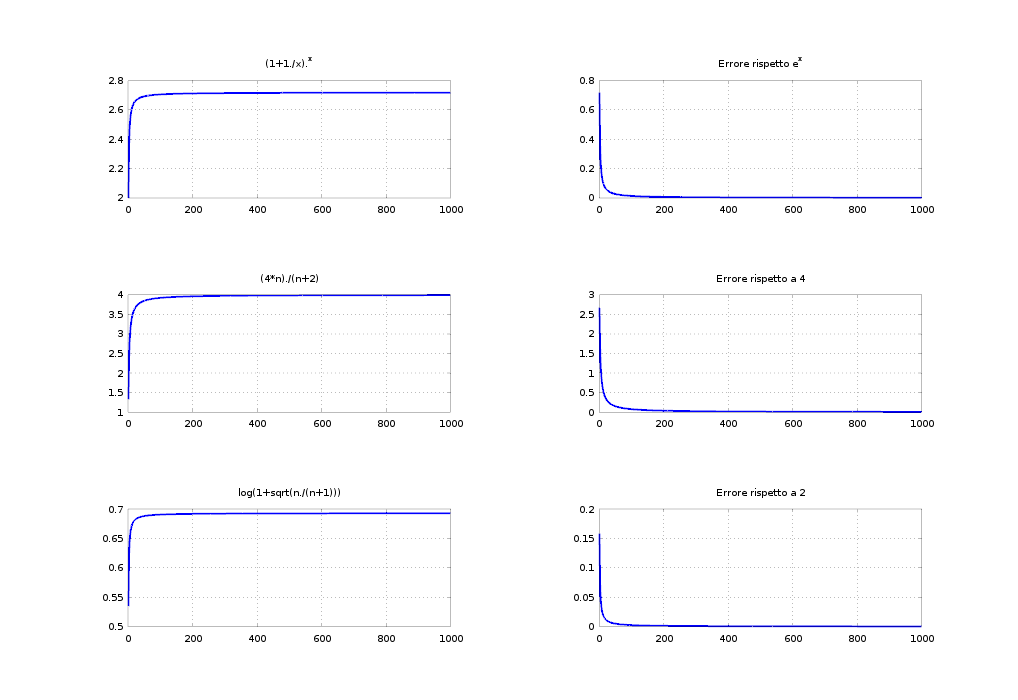
\includegraphics[scale=0.6]{ex23.png}}


%%%%%%%%%%%%%%%%%%%%%%%%%%%%%%%%%%%%%%%%%%%%%%%%%%%%%%%%%%%%%%%%%%%%%%%%%%%%%%%%%%%%%
\newpage
\subsection{ Esercizio 4}
\begin{lstlisting}
f1 = inline("sqrt(x.^2+1)-x");
f2 = inline("x.*sqrt(x.^2+1)-x.^2");
f3 = inline("x./(sqrt(x.^2+1)+x)");

x = 1:2:1000;

y1 = f1(x);
y2 = f2(x);
y3 = f3(x);


subplot(3,1,1)
  plot(x,y1,'linewidth',2);
  title("sqrt(x.^2+1)-x");
  grid on
subplot(3,1,2)
  plot(x,y2,'linewidth',2);
  title("x.*sqrt(x.^2+1)-x.^2")
  grid on
subplot(3,1,3)
  plot(x,y3,'linewidth',2);
  title("x./(sqrt(x.^2+1)+x)")
  grid on

\end{lstlisting}

\centerline{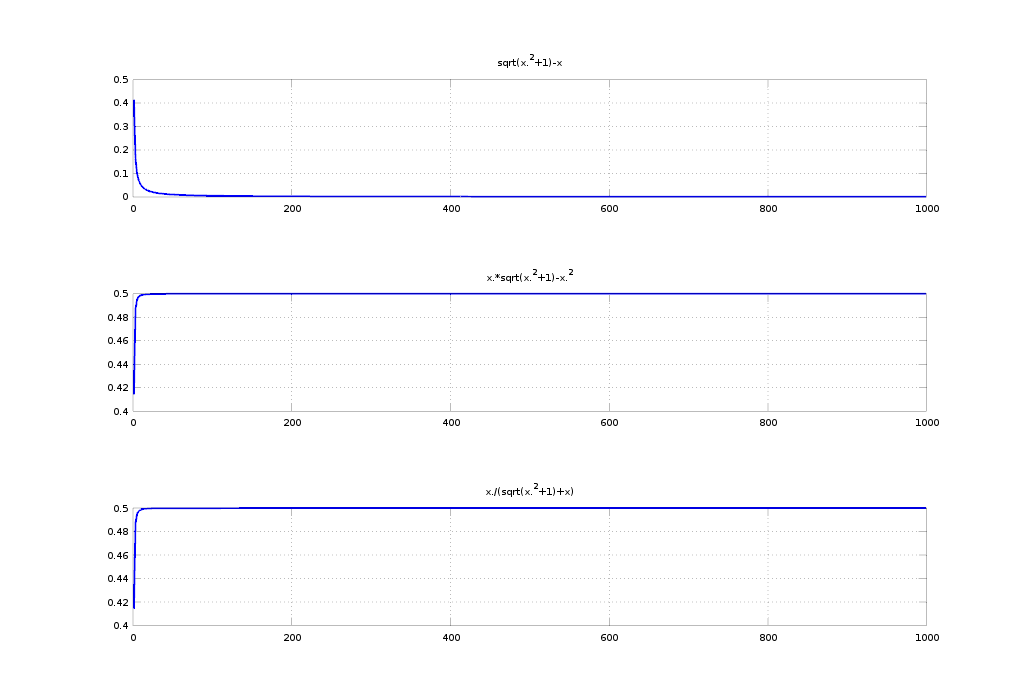
\includegraphics[scale=0.6]{ex24.png}}


%%%%%%%%%%%%%%%%%%%%%%%%%%%%%%%%%%%%%%%%%%%%%%%%%%%%%%%%%%%%%%%%%%%%%%%%%%%%%%%%%%%%%
\newpage
\subsection{ Esercizio 5}
\begin{lstlisting}
d0 = -2*ones(1,9);
d1 = ones(1,8);

A = diag(d0) + diag(d1,1) + diag(d1,-1);
A([3,6],:) = A([6,3],:);
A(:,[1,4]) = A(:,[4,1]);
\end{lstlisting}


%%%%%%%%%%%%%%%%%%%%%%%%%%%%%%%%%%%%%%%%%%%%%%%%%%%%%%%%%%%%%%%%%%%%%%%%%%%%%%%%%%%%%
\newpage
\subsection{ Esercizio 6}
\begin{lstlisting}
x = [1:12];
A = [x([1:4]);x([5:8]);x([9:12])];
size(A)
B = A.*A
B = A*A
B = A'*A
A(1:2,4)
A(:,3)
A(1:2,:)
A(:,[2 4])
A([2 3 3])
A(3,2)=A(1,1)
A(1:2,4) = zeros(2,1);
A(2,:) = A(2,:)-A(2,1)/A(1,1)*A(1,:);
\end{lstlisting}


%%%%%%%%%%%%%%%%%%%%%%%%%%%%%%%%%%%%%%%%%%%%%%%%%%%%%%%%%%%%%%%%%%%%%%%%%%%%%%%%%%%%%
\newpage
\subsection{ Esercizio 7}
\begin{lstlisting}
a = ones(1,8)
A = [];
for b= 1:8
 A(b,:) = b*a;
endfor

S = triu(A)
L = tril(A)

for i=1:size(S)
  S(i,i) = 0;
  L(i,i) = 1;
endfor

d0 = diag(A);
d1 = diag(A,1);
d_1 = diag(A,-1);

B1 = diag(d0) + diag(d1,1) + diag(d_1,-1);
B2 = diag(d0) + diag(d1,1);
B3 = diag(d0) + diag(d_1,-1);


\end{lstlisting}


%%%%%%%%%%%%%%%%%%%%%%%%%%%%%%%%%%%%%%%%%%%%%%%%%%%%%%%%%%%%%%%%%%%%%%%%%%%%%%%%%%%%%
\newpage
\subsection{ Esercizio 8 \\ Sviluppo di una funzione matlab per il calcolo delle radici di un'equazione di quarto grado}
\begin{lstlisting}
function X = lp_root(alpha)

  b = (1+10^(2*alpha))/10^alpha;
  t1 = (b + sqrt(b^2-4))/2;
  t2 = (b - sqrt(b^2-4))/2;

  x1 = -sqrt(t1);
  x2 = -sqrt(t2);
  x3 =  sqrt(t1);
  x4 =  sqrt(t2);

  X = [ x1, x2, x3, x4 ];

endfunction


A = [];

for i=1:10
  A = [ A ; lp_root(i) ];
endfor


B = [];

for i=1:10
  B = [ B ; roots([ 1, 0, -((1+10^(2*i))/10^i), 0, 1])' ];
endfor


for i=1:10
  A(i,:) = sort(A(i,:));
  B(i,:) = sort(B(i,:));
endfor

E1 = abs(A-B)./A;
E2 = abs(A-B)./B;


\end{lstlisting}



%%%%%%%%%%%%%%%%%%%%%%%%%%%%%%%%%%%%%%%%%%%%%%%%%%%%%%%%%%%%%%%%%%%%%%%%%%%%%%%%%%%%%
\newpage
\subsection{ Esercizio 9}
\begin{lstlisting}
\end{lstlisting}

%%%%%%%%%%%%%%%%%%%%%%%%%%%%%%%%%%%%%%%%%%%%%%%%%%%%%%%%%%%%%%%%%%%%%%%%%%%%%%%%%%%%%
%%%%%%%%%%%%%%%%%%%%%%%%%%%%%%%%%%%%%%%%%%%%%%%%%%%%%%%%%%%%%%%%%%%%%%%%%%%%%%%%%%%%%
\newpage
\section{ Esercitazione 3}


%%%%%%%%%%%%%%%%%%%%%%%%%%%%%%%%%%%%%%%%%%%%%%%%%%%%%%%%%%%%%%%%%%%%%%%%%%%%%%%%%%%%%
\subsection{ Esercizio 1}
\begin{lstlisting}
x = -5:1:9;
M = max(x)
M =  9
m = min(x)
m = -5
abM = max(abs(x))
abM =  9
abm = min(abs(x))
abm = 0
S = sum(x)
S =  30
abS = sum(abs(x))
abS =  60

\end{lstlisting}


%%%%%%%%%%%%%%%%%%%%%%%%%%%%%%%%%%%%%%%%%%%%%%%%%%%%%%%%%%%%%%%%%%%%%%%%%%%%%%%%%%%%%
\newpage
\subsection{ Esercizio 2 \\ Calcolo di $\lim_{x\to 0}{\frac{(x+1)^2-1}{x}}$ e $\lim_{x\to 0}{x+2}$}
\begin{lstlisting}
  f1 = inline (" ((x+1).^2 -1)./x ");
f2 = inline (" x+2 ");

x = 1:-0.001:0;

y1 = f1(x);
y2 = f2(x);

subplot(2,1,1) 
  plot(x,y1,'linewidth',2);
  title(" ((x+1)^2 -1 )/x ");
  grid on
subplot(2,1,2)
  plot(x,y2,'linewidth',2);
  title(" x+2 ")
  grid on
\end{lstlisting}


\begin{lstlisting}
f1 = inline (" ((x+1).^2 -1)./x ");
f2 = inline (" x+2 ");

x = 1:-0.001:0;

y1 = f1(x);
y2 = f2(x);

subplot(2,1,1) 
  plot(x,y1,'linewidth',2);
  title(" ((x+1)^2 -1 )/x ");
subplot(2,1,2)
  plot(x,y2,'linewidth',2);
  title(" x+2 ")
\end{lstlisting}


\centerline{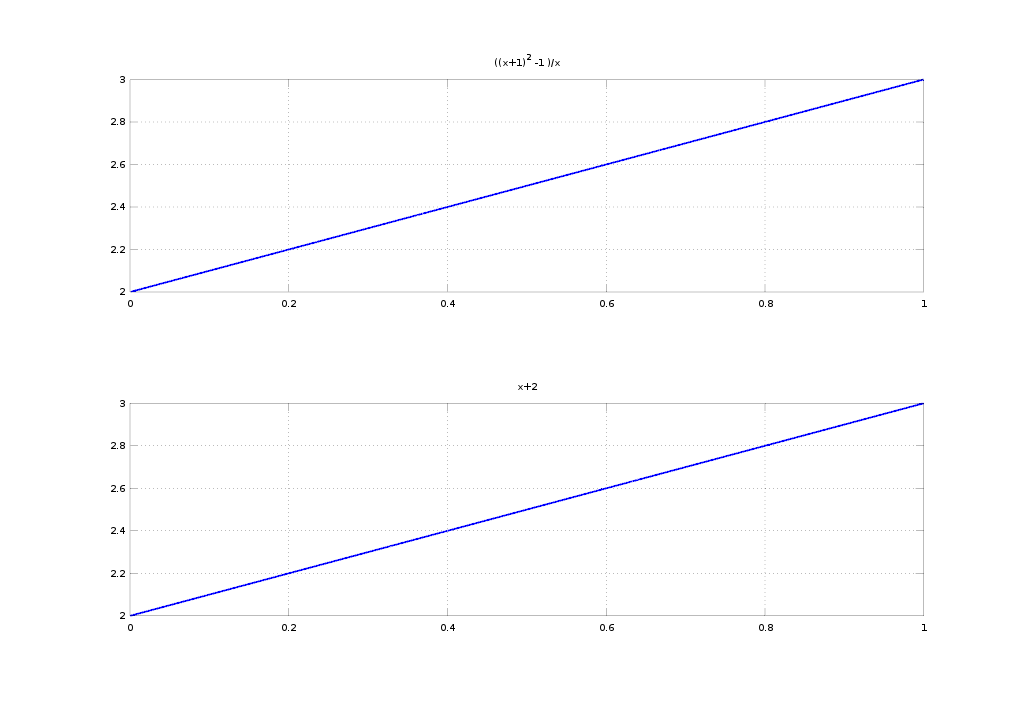
\includegraphics[scale=0.6]{ex32.png}}


%%%%%%%%%%%%%%%%%%%%%%%%%%%%%%%%%%%%%%%%%%%%%%%%%%%%%%%%%%%%%%%%%%%%%%%%%%%%%%%%%%%%%
\newpage
\subsection{ Esercizio 3 \\ Sviluppo di Taylor per il calcolo di $e^x$}
\begin{lstlisting}
% e^x = 1 + x^2/2! + x^3/3! + ....
% Calcolare e^-9 stabilizzando la 6 cifra dopo la virgola


x1 = [];
x2 = [];

err = 10^-6;

my_e1 = 1;
x = -9;
i = 1;
while ( abs(e^-9 - my_e1) > err )
 my_e1 = my_e1 + x^i/factorial(i);
 i = i+1;
 x1 = [ x1 , my_e1 ];
endwhile

e2 = 1;
my_e2 = 1;
x = 9;
i = 1;
while ( abs(e^-9 - my_e2) > err )
  e2 = e2 + x^i/factorial(i);
  my_e2 = 1/e2;
  i = i+1;
  x2 = [ x2, my_e2 ];
endwhile 
 




% Calcolo degli errori relativi
%  Calcolati sulla somma dei primi n termini


err_rel1 = [];
for i=1:size(x1)(2)
  err_rel1 = [ err_rel1 , abs(x1(i) - exp(-9))/exp(-9) ];
endfor

err_rel2 = [];
for i=1:size(x2)(2)
  err_rel2 = [ err_rel2 , abs(x2(i) - exp(-9))/exp(-9) ]; 
endfor


a1 = 1:size(x1)(2);
a2 = 1:size(x2)(2);

subplot(2,1,1)
plot(a1,x1,'linewidth',2);

subplot(2,1,2)
plot(a2,x2,'linewidth',2);
\end{lstlisting}


\centerline{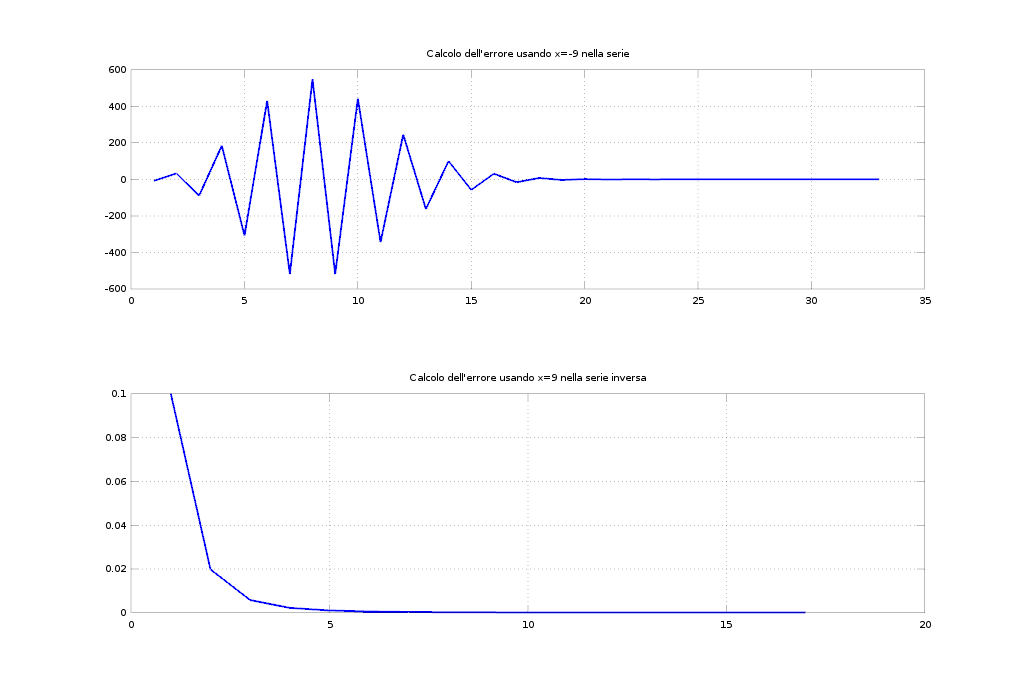
\includegraphics[scale=0.6]{ex33.png}}


%%%%%%%%%%%%%%%%%%%%%%%%%%%%%%%%%%%%%%%%%%%%%%%%%%%%%%%%%%%%%%%%%%%%%%%%%%%%%%%%%%%%%
\newpage
\subsection{ Esercizio 4 \\ Approssimazioni della derivata di $e^x$ nel punto $x=1$}
\begin{lstlisting}
h = [];

for a=1:1:20
  h = [ h, 10^(-a) ];
endfor

x = 1;
app1 = (exp(x+h)-exp(x))./h;
app2 = (exp(x+h)-exp(x-h))./(2*h);

analitic1 = abs((app1 - exp(1)));
analitic2 = abs((app2 - exp(1)));

tab = [ h', analitic1', analitic2' ]

#{
   1.0000e-01   1.4056e-01   4.5327e-03
   1.0000e-02   1.3637e-02   4.5305e-05
   1.0000e-03   1.3596e-03   4.5305e-07
   1.0000e-04   1.3592e-04   4.5306e-09
   1.0000e-05   1.3591e-05   5.8587e-11
   1.0000e-06   1.3590e-06   1.6346e-10
   1.0000e-07   1.3995e-07   5.8587e-11
   1.0000e-08   6.6028e-09   6.6028e-09
   1.0000e-09   2.1544e-07   6.6028e-09
   1.0000e-10   1.5477e-06   6.7274e-07
   1.0000e-11   3.2634e-05   1.0429e-05
   1.0000e-12   4.3231e-04   2.1027e-04
   1.0000e-13   4.5586e-04   4.5586e-04
   1.0000e-14   9.3376e-03   9.3376e-03
   1.0000e-15   3.9034e-01   1.6830e-01
   1.0000e-16   2.7183e+00   2.7183e+00
   1.0000e-17   2.7183e+00   2.7183e+00
   1.0000e-18   2.7183e+00   2.7183e+00
   1.0000e-19   2.7183e+00   2.7183e+00
   1.0000e-20   2.7183e+00   2.7183e+00
#}


\end{lstlisting}


%%%%%%%%%%%%%%%%%%%%%%%%%%%%%%%%%%%%%%%%%%%%%%%%%%%%%%%%%%%%%%%%%%%%%%%%%%%%%%%%%%%%%
\newpage
\subsection{ Esercizio 5}
\begin{lstlisting}
H = hilb(10);
x = ones(10,1);

b = H*x;

x1 = H\b;

z = [ 0.001, zeros(1,size(b)-1)]'

c = b+z ;

y = H\c;

err = norm(x-y)/norm(x)

err =  4852.2

\end{lstlisting}


%%%%%%%%%%%%%%%%%%%%%%%%%%%%%%%%%%%%%%%%%%%%%%%%%%%%%%%%%%%%%%%%%%%%%%%%%%%%%%%%%%%%%
%%%%%%%%%%%%%%%%%%%%%%%%%%%%%%%%%%%%%%%%%%%%%%%%%%%%%%%%%%%%%%%%%%%%%%%%%%%%%%%%%%%%%
\newpage
\section{ Esercitazione 4}


%%%%%%%%%%%%%%%%%%%%%%%%%%%%%%%%%%%%%%%%%%%%%%%%%%%%%%%%%%%%%%%%%%%%%%%%%%%%%%%%%%%%%
\subsection{ Esercizio 1 \\ Interpolazione con Vandermonde e perturbazione dei dati}
\begin{lstlisting}
x10 = linspace(-1,1,10);
x15 = linspace(-1,1,15);
x20 = linspace(-1,1,20);

V10 = vander(x10);
V15 = vander(x15); 
V20 = vander(x20);

f = inline(" exp(x)+1 ");

% I bi sono i coefficienti della funzione calcolati nei nodi 
%   mi servono ad imporre le condizioni di interpolazione.
b10 = f(x10)';
b15 = f(x15)';
b20 = f(x20)';

% I sistemi sarebbero genericamente Vx = b, devo trovare x
%   che per comodit\'{a} chiamer\'{o} a, il vettore dei coefficienti.


% Coefficienti del polinomio  
a10 = V10\b10;
a15 = V15\b15;
a20 = V20\b20;


eps = [];
for i=1:20
 eps = [ eps, (-1)^(i)*10^(-5) ];
endfor

b10_1 = b10 + eps([1:10])';
b15_1 = b15 + eps([1:15])';
b20_1 = b20 + eps([1:20])';


% Coefficienti polinomio perturbato
a10_1 = V10\b10_1;
a15_1 = V15\b15_1;
a20_1 = V20\b20_1;




% Ricordiamo che Un polinomio in Matlab `e dato da un vettore che contiene 
%   i sui coefficienti ordinati da an  fino ad a0.



a10 = fliplr(a10);
a15 = fliplr(a15);
a20 = fliplr(a20);
a10_1 = fliplr(a10_1);
a15_1 = fliplr(a15_1);
a20_1 = fliplr(a20_1);


% Uso x20 per valutare i polinomi 
y10 = polyval(a10,x20);
y15 = polyval(a15,x20);
y20= polyval(a20,x20);
y10_1 = polyval(a10_1,x20);
y15_1 = polyval(a15_1,x20);
y20_1 = polyval(a20_1,x20);

,'linewidth',2,


subplot(3,1,1)
 plot(x20,y10,'linewidth',2,'*',x20,y10_1,'linewidth',2,'g'); 
 grid on
 legend("Polinomio interpolante","Polinomio interpolante perturbato");
 title("Polinomi di 10 grado");
subplot(3,1,2)
 plot(x20,y15,'linewidth',2,'*',x20,y15_1,'linewidth',2,'g'); 
 grid on
 legend("Polinomio interpolante","Polinomio interpolante perturbato");
 title("Polinomi di 15 grado");
subplot(3,1,3)
 plot(x20,y20,'linewidth',2,'*',x20,y20_1,'linewidth',2,'g'); 
 grid on 
 legend("Polinomio interpolante","Polinomio interpolante perturbato");
 title("Polinomi di 20 grado");

maxa10 = max(abs(a10 - a10_1));
maxa15 = max(abs(a15 - a15_1));
maxa20 = max(abs(a20 - a20_1));

t = linspace(-1,1,101);

pt10   = polyval(a10,t);
pt10_1 = polyval(a10_1,t);
pt15   = polyval(a15,t);
pt15_1 = polyval(a15_1,t);
pt20   = polyval(a20,t);
pt20_1 = polyval(a20_1,t);


maxp10 = max(abs(pt10-pt10_1)); 
maxp15 = max(abs(pt15-pt15_1));
maxp20 = max(abs(pt20-pt20_1));


\end{lstlisting}


\centerline{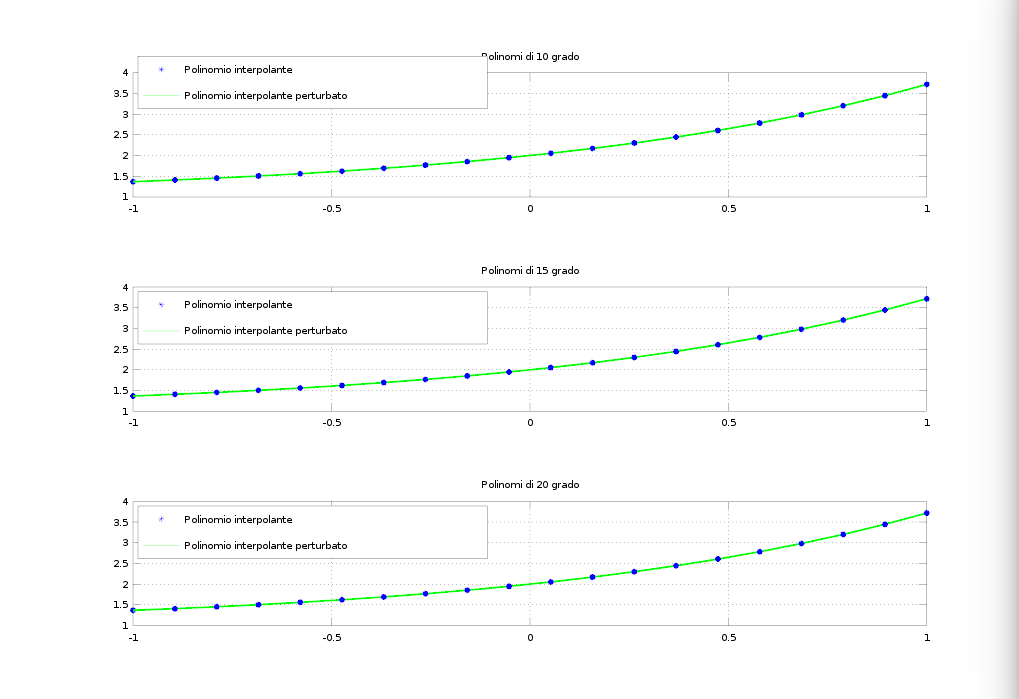
\includegraphics[scale=0.6]{ex41.png}}


%%%%%%%%%%%%%%%%%%%%%%%%%%%%%%%%%%%%%%%%%%%%%%%%%%%%%%%%%%%%%%%%%%%%%%%%%%%%%%%%%%%%%
\newpage
\subsection{ Esercizio 2}
\begin{lstlisting}
A = hilb(1000);
B = rand(1000);

x = ones(1000,1);
y = ones(1000,1);

% Ax = b;
% By = c;

b = A*x;
c = B*y;

x1 = A\x;
y1 = B\y;

%  Calcolare gli errori relativi tra b,c b1 e c1
%   rapportandoli al numero di condizionamento di A e B

Ka = cond(A);
Kb = cond(B);


err_relx = norm(x-x1)/norm(x);
err_rely = norm(y-y1)/norm(y);

\end{lstlisting}


%%%%%%%%%%%%%%%%%%%%%%%%%%%%%%%%%%%%%%%%%%%%%%%%%%%%%%%%%%%%%%%%%%%%%%%%%%%%%%%%%%%%%
%%%%%%%%%%%%%%%%%%%%%%%%%%%%%%%%%%%%%%%%%%%%%%%%%%%%%%%%%%%%%%%%%%%%%%%%%%%%%%%%%%%%%
\newpage
\section{ Esercitazione 5}


%%%%%%%%%%%%%%%%%%%%%%%%%%%%%%%%%%%%%%%%%%%%%%%%%%%%%%%%%%%%%%%%%%%%%%%%%%%%%%%%%%%%%
\subsection\protect{ Esercizio 1 \\ Rappresentazione grafica di funzioni} 

\begin{flushleft}
\vspace{0.2cm}
$f(x) = 2sin(8x)-ln(x^2+1)$ \\
\vspace{0.4cm}
$g(x)=\begin{cases}x^2 & x < 3 \\ 9 & x > 3\end{cases} $
\end{flushleft}

\begin{lstlisting}
%%%%%% PARTE a %%%%%%%
function plot_f(a,b)

 f = inline(" 2*sin(8*x) - log(x.^2+1) ");

 if ( a < b )
    c = a;
    a = b; 
    b = c;
  endif
 
  x = linspace(a,b,(a-b)*100);

  y = f(x);   

  plot(x,y,'r');
  xlabel(" decomposition ");
  ylabel(" 2*sin(8*x) - ln(x.^2+1) ");
  grid on;

endfunction

plot_f(-6,6)

%%%%%% PARTE a %%%%%%%

x1 = linspace(2,3,50);
x2 = linspace(3,4,50);

g1 = inline('x.^2');
plot(x1,g1(x1));
  
hold on
   
g2 = 9;
plot(x2,g2);  

\end{lstlisting}


\centerline{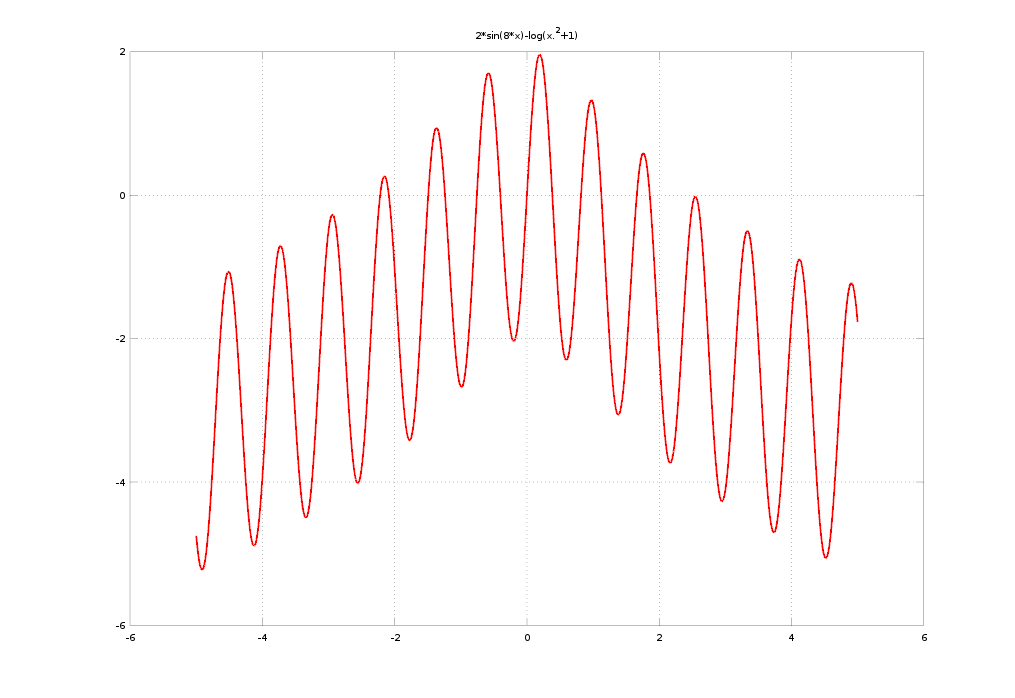
\includegraphics[scale=0.6]{ex51a.png}}
\centerline{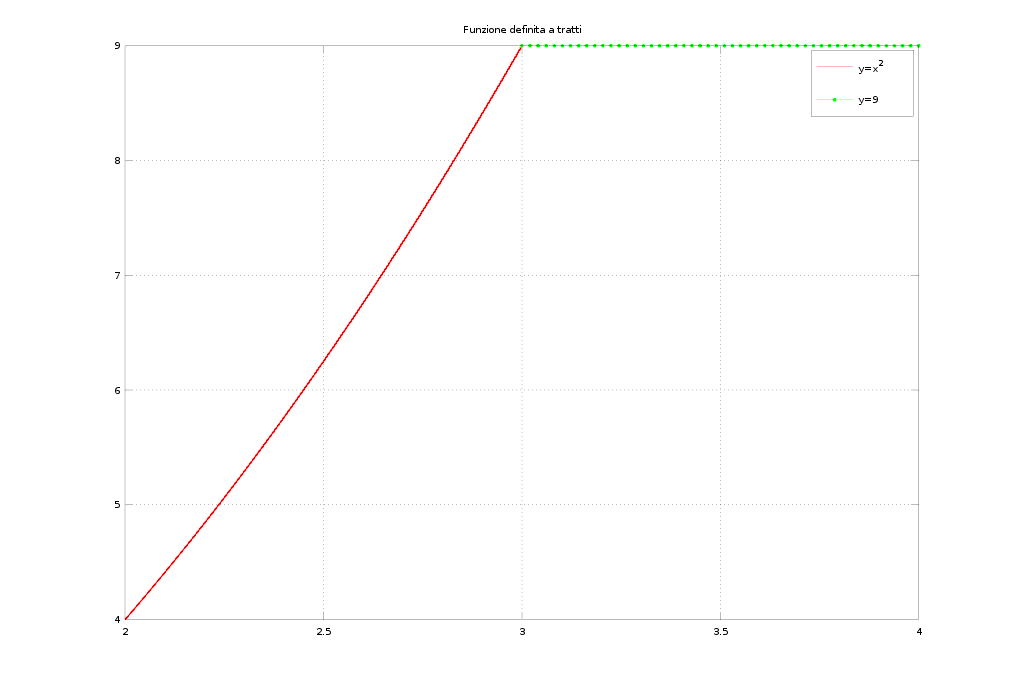
\includegraphics[scale=0.6]{ex51b.png}}


%%%%%%%%%%%%%%%%%%%%%%%%%%%%%%%%%%%%%%%%%%%%%%%%%%%%%%%%%%%%%%%%%%%%%%%%%%%%%%%%%%%%%
\newpage
\subsection{ Esercizio 2}
\begin{lstlisting}

\end{lstlisting}


%%%%%%%%%%%%%%%%%%%%%%%%%%%%%%%%%%%%%%%%%%%%%%%%%%%%%%%%%%%%%%%%%%%%%%%%%%%%%%%%%%%%%
\newpage
\subsection{ Esercizio 3}
\begin{lstlisting}
function [x,y] = m_calc(m)
  m = abs(m);
  x1 = linspace(-m,0,50);
  x2 = linspace( 0,m,50);
  
  y1 =  (m-(x1.^2)./m).^m ;
  y2 =  ((x2.^2)./m+m).^m ;

  x = [ x1 x2 ];
  y = [ y1 y2 ];

endfunction

x=[];
y=[];

A = [];
for i=1:6
 [ x,y ] = m_calc(i);
 A = [ [ x, y ] ; A];
 semilogy(x,y);
 %legend([ " m = " num2str(i) ] );
 hold on
endfor



figure 2
for i=1:6
  subplot(2,3,i)
  semilogy(A(i,1:100),A(i,101:200));
  title([ " m = " num2str(i) ]);
  ylabel(" log scale ");
endfor
\end{lstlisting}

\newpage
\centerline{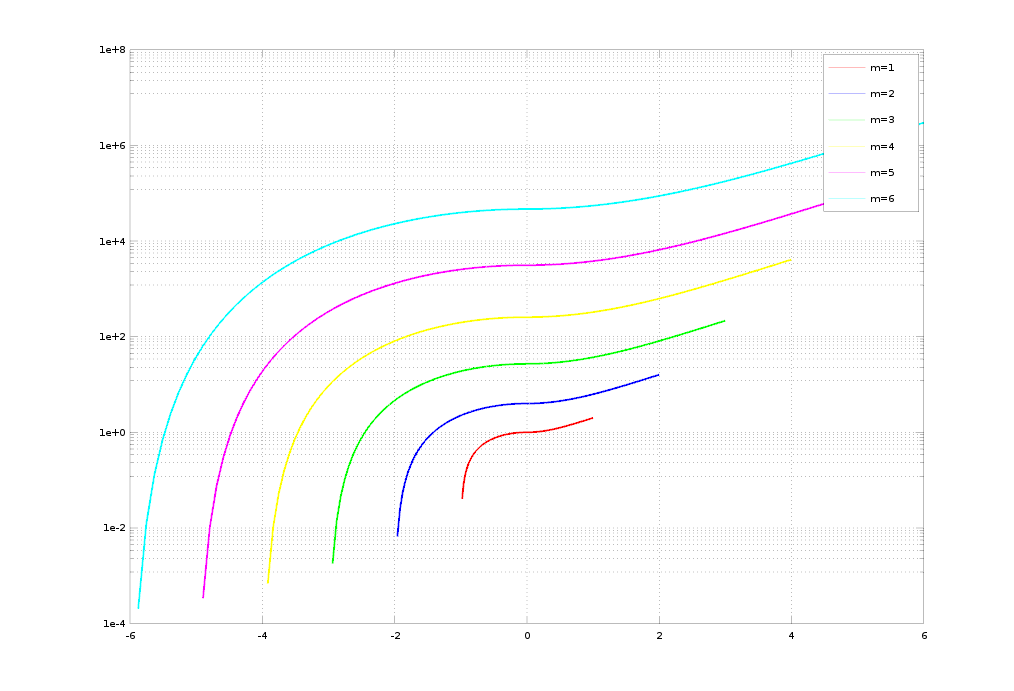
\includegraphics[scale=0.4]{ex53a.png}}
\centerline{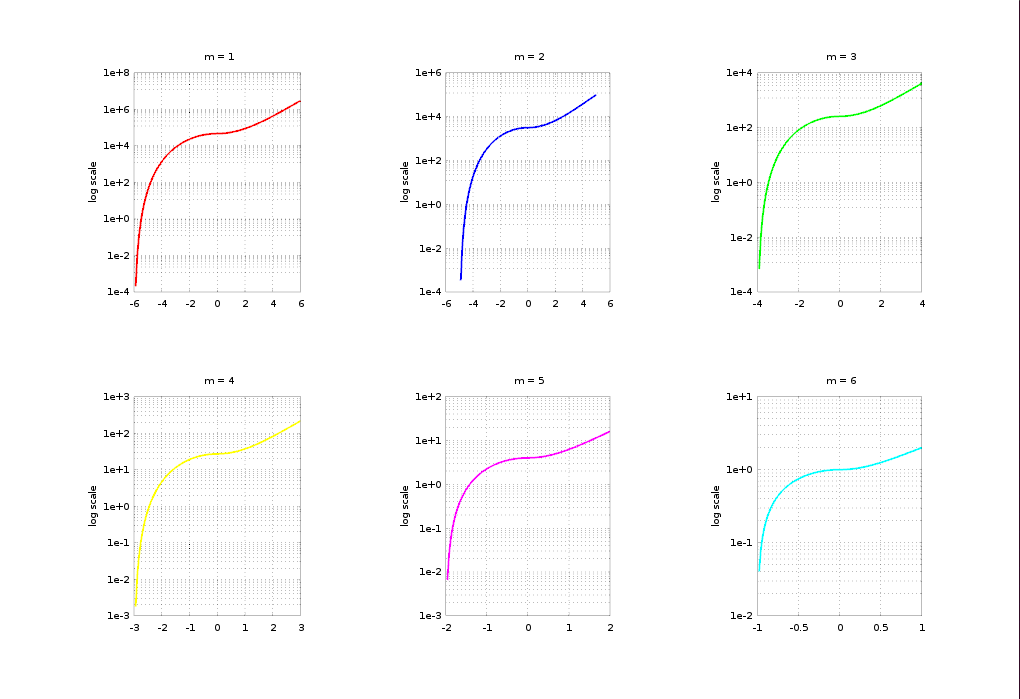
\includegraphics[scale=0.4]{ex53b.png}}


%%%%%%%%%%%%%%%%%%%%%%%%%%%%%%%%%%%%%%%%%%%%%%%%%%%%%%%%%%%%%%%%%%%%%%%%%%%%%%%%%%%%%
\newpage
\subsection{ Esercizio 4 \\ Risoluzione di sistemi lineari a matrice tridiagonale}
\begin{lstlisting}
% Risoluzione di sistemi lineari con matrici tridiagonali
%  Utilizzo la fattorizzazione LU per la matrice A e poi 
%  risolvo il sistema che ne consegue.


A = diag(ones(1,5));
A = A + diag(ones(1,4),1)*3;
A = A + diag(ones(1,4),-1)*5;

% Fattorizzazione LU per matrici tridiagonali.
  % conditio sine qua non A deve essere tridiagonale.
function [ L, U ] = tridiag_fatt(A)
  a = diag(A);
  c = diag(A,1);
  b = diag(A,-1);

  % Calcolo dei determinanti dei minori
  %  NB d(n) = det(A)

  d = ones(1,size(a)+1);
  d(1) = 1;
  d(2) = a(1);
  for i=2:size(a)
    d(i+1) =  (a(i)*d(i) - b(i-1)*c(i-1)*d(i-1));
  endfor


  % diagonale inferiore di L
  l = ones(1,size(a)-1);
  % diagonale principale di U
  u = ones(1,size(a));

  for i=1:size(a)-1
   l(i) = l(i)*( b(i)*d(i)/d(i+1) );
  endfor

  for i=1:size(a)
   u(i) = d(i+1)/d(i);
  endfor

  % Ora posso calcolare le due matrici L ed U
  
  L = diag(ones(1,size(a))) + diag(l,-1);
  U = diag(u) + diag(c,1);

endfunction


[ L,U ] = tridiag_fatt(A);
b = [ 1,2,3,4,5 ]';
%% Algoritmo di risoluzione
%   Ax = b
%   A  = LU
%   LUx = b
%
%   Ly = b
%   Ux = y
%   
%
%   x \'{e} la mia soluzione finale  


% Diagonale inferiore di L
 bl = diag(L,-1);

% Diagonale principale di U
 au = diag(U);

% Diagonale superiore di U
 cu = diag(U,1);

n = size(L)(1);


x_sure = A\b

y = ones(1,n);
x = ones(1,n);Y


% Risoluzione di Ly = b
y(1) = b(1);
for i=2:n
  y(i) = b(i) - bl(i-1)*y(i-1);
endfor


% Risoluzione di Ux = y
x(n) = y(n)/au(n);
for i=n-1:-1:1
  x(i) = (y(i-1)-cu(i)*x(i+1))/cu(i);
endfor
\end{lstlisting}


%%%%%%%%%%%%%%%%%%%%%%%%%%%%%%%%%%%%%%%%%%%%%%%%%%%%%%%%%%%%%%%%%%%%%%%%%%%%%%%%%%%%%
\newpage
\subsection{ Esercizio 5}
\begin{lstlisting}
% funzione per matrice bidiagonale del tipo
%   A = diag(ones(1,n)) + diag(2*ones(1,n-1),1);

function [ inv_A ] = inv_bidiag(A);

% Calcolo l'inversa con il metodo di Gauss Giordan


% n = numero di righe di A
n = size(A)(1);


AI = [ A , eye(size(A)(2)) ];


for r=n:-1:2
  AI(r-1,:) = AI(r-1,:)-2*AI(r,:);
endfor

inv_A = AI(:,size(AI)(2)/2+1:size(AI)(2));


endfunction


a1=1:10;
c1=11:19;

A = diag(a1) + diag(c1,1) + diag(c1,-1);

% A deve essere tridiagonale
function [ B ] = tri_fact(A)

  n = size(A)(2);
  p = ones(1,n);
  q = ones(1,n-1);
  a = diag(A);
  c = diag(A,-1);

  p(1) = sqrt(a(1));

  for i=2:n
    q(i-1) = c(i-1)./p(i-1);
    p(i) = sqrt(a(i)-q(i-1).^2);
  endfor

  B = diag(p) + diag(q,-1);

endfunction

B = tri_fact(A);

A1 = B*B';

\end{lstlisting}


%%%%%%%%%%%%%%%%%%%%%%%%%%%%%%%%%%%%%%%%%%%%%%%%%%%%%%%%%%%%%%%%%%%%%%%%%%%%%%%%%%%%%
\newpage
\subsection{ Esercizio 6}
\begin{lstlisting}
t = 1:6;
y = [ 0.5,0.8,0.7,0.3,0.1,0.4 ]

f = inline(' 1 + sin(2*pi*x/6) + cos(2*pi*x/6) ');


A = [];
for i=1:6
  A = [ A ; [ 1, sin(2*pi*i/6), cos(2*pi*i/6) ] ];
endfor

a = A\y';

a = fliplr(a);

p = polyval(a,t);

A

\end{lstlisting}


%%%%%%%%%%%%%%%%%%%%%%%%%%%%%%%%%%%%%%%%%%%%%%%%%%%%%%%%%%%%%%%%%%%%%%%%%%%%%%%%%%%%%
\newpage
\subsection{ Esercizio 7}
\begin{lstlisting}
a1=1:10;
c1=11:19;

A = diag(a1) + diag(c1,1) + diag(c1,-1);

% A deve essere tridiagonale
function [ B ] = tri_fact(A)

  n = size(A)(2);
  p = ones(1,n);
  q = ones(1,n-1);
  a = diag(A);
  c = diag(A,-1);

  p(1) = sqrt(a(1));

  for i=2:n
    q(i-1) = c(i-1)./p(i-1);
    p(i) = sqrt(a(i)-q(i-1).^2);
  endfor

  B = diag(p) + diag(q,-1);

endfunction

B = tri_fact(A);

A1 = B*B';

\end{lstlisting}


%%%%%%%%%%%%%%%%%%%%%%%%%%%%%%%%%%%%%%%%%%%%%%%%%%%%%%%%%%%%%%%%%%%%%%%%%%%%%%%%%%%%%
\newpage
\subsection{ Esercizio 8 \\ Approssimazione di $\pi$ mediante troncata di una serie}
\begin{lstlisting}
tr = inline("16^(-x)*(4/(8*x+1) - 2/(8*x+4) - 1/(8*x+5) - 1/(8*x+6))");

p0 = (4-1/2-1/5-1/6);

p_i = p0*ones(1,100);
	 

for a=2:100
  for b=1:a
    p_i(a) = p_i(a) + tr(b);
  endfor
endfor

% converge velocemente a pi

real_pi = ones(1,100)*pi;
err = abs(real_pi - p_i);

% alla decima iterazione l'errore in format long risulta essere nullo

plot(1:10,err(1:1:10),'linewidth',2,'r');
grid on
title("Andamento dell'errore di approssimazione");

\end{lstlisting}



\centerline{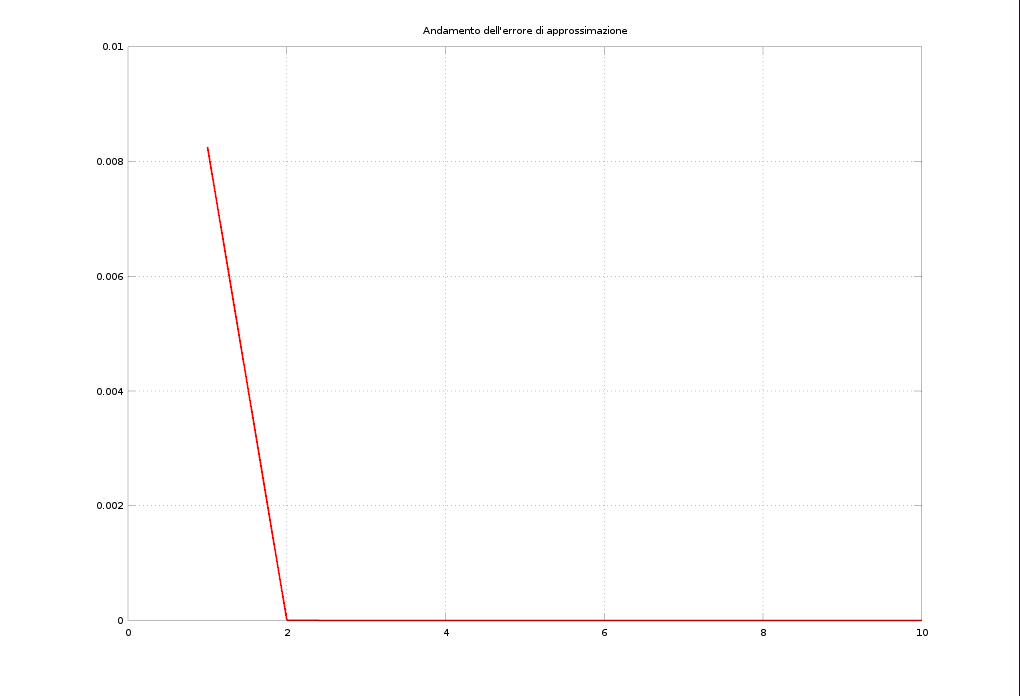
\includegraphics[scale=0.6]{ex58.png}}


%%%%%%%%%%%%%%%%%%%%%%%%%%%%%%%%%%%%%%%%%%%%%%%%%%%%%%%%%%%%%%%%%%%%%%%%%%%%%%%%%%%%%
%%%%%%%%%%%%%%%%%%%%%%%%%%%%%%%%%%%%%%%%%%%%%%%%%%%%%%%%%%%%%%%%%%%%%%%%%%%%%%%%%%%%%
\newpage
\section{ Esercitazione 6}


%%%%%%%%%%%%%%%%%%%%%%%%%%%%%%%%%%%%%%%%%%%%%%%%%%%%%%%%%%%%%%%%%%%%%%%%%%%%%%%%%%%%%
\subsection{ Esercizio 1}

\begin{lstlisting}
 %months = [ 'G','F','M','A','M','J','L','A','S','O','N','D']
 %set(gca,'XtickLabel',months)
 x=1:12;
 y=[12.51, 13.05, 11.7, 9.26, 8.3, 6.25, 5.34, 4.59, 5.14, 6.36, 10.31, 13.88]


 xx=linspace(1,12,1201);


 % spline lineare  
 % se il campo " metodo " viene omesso di default viene usata
 %  l'interpolazione lineare, ovvero le spline lineari
 
 yyl = interp1(x,y,xx);


 % interpolazione polinomiale
 % comando polifit

 coeff_yyp = polyfit(x,y,11);
 yyp = polyval(coeff_yyp,xx);

 % spline cubica
 
 yyc = interp1(x,y,xx,'spline');

 
 % plotting

 plot(x,y,'o',xx,yyl,'g',xx,yyp,'b',xx,yyc,'r');
 grid on
 ylabel("Portata [m^3/sec]");
 xlabel("Months");
 title("Confronto calcolo della portata tramite tre metodi di interpolazione");

 legend(" Nodi "," interpolazione lineare a tratti "," interpolazione polinomiale "," interpolazione cubica a tratti ");


\end{lstlisting}


\centerline{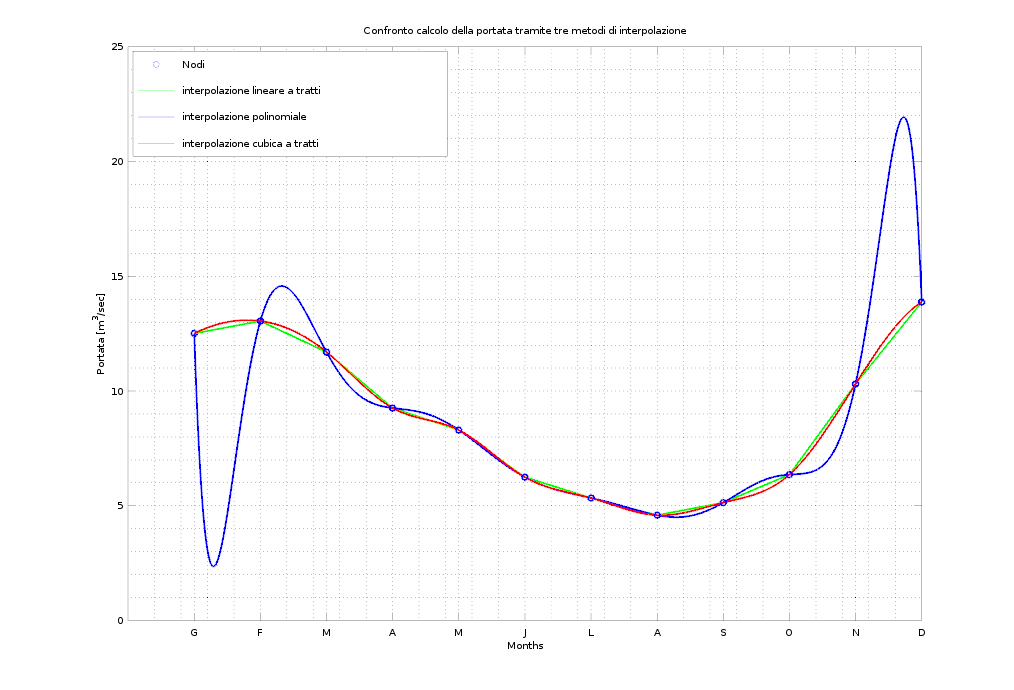
\includegraphics[scale=0.6]{ex61.png}}


%%%%%%%%%%%%%%%%%%%%%%%%%%%%%%%%%%%%%%%%%%%%%%%%%%%%%%%%%%%%%%%%%%%%%%%%%%%%%%%%%%%%%
\newpage
\subsection{ Esercizio 2}
\begin{lstlisting}
f = inline("-(x-5).*log(x)./x.^2");
x = 1:0.5:5;
y = f(x);


xx = linspace(1,5,500);

% comando interp1 per interpolazione a tratti lineare

yyl = interp1(x,y,xx,'linear'); 

% comando interp1 per interpolazione a tratti cubica


yyi = interp1(x,y,xx,'cubic');


% comando spline per interpolazione a tratti

pps = spline(x,y);
yys = ppval(pps,xx);


% plotting

plot(x,y,'linewidth',2,'o',xx,yyi,'linewidth',2,'g',xx,yys,'linewidth',2,'r',xx,yyl,'linewidth',2,'b');
legend(" Nodi ", " Interp1 Spline Cubica ", " Spline Cubica ", " Interp1 Spline Lineare");
grid on

% Errori
% Valori della funzione nei punti xx

yyreal = f(xx);

% confrontiamo i valori della funzione con quelli approssimati

err_interp_lineare = abs(yyreal-yyl);
err_interp_cubica  = abs(yyreal-yys);
err_interp_spline  = abs(yyreal-yys);


figure 2 

plot(xx,err_interp_cubica,'linewidth',2,'g',xx,err_interp_spline,'linewidth',2,'o',xx,err_interp_lineare,'linewidth',2,'r');
legend(" Interp1 Spline Cubica ", " Spline Cubica ", " Interp1 Spline Lineare");
grid on


% La migliore funzione interpolante risulta essere, all'analisi degli errori, la spline cubica.
%  Gli errori della spline cubica calcolati con la funzione spline e quelli calcolati con la funzione
%  interpl(xx,yy,'spline') risultano essere praticamente sovrapposti nel grafico, possiamo concludere quindi che siano
%  entrambi metodi appropriati per il calcolo della funzione interpolante 
 

\end{lstlisting}



\centerline{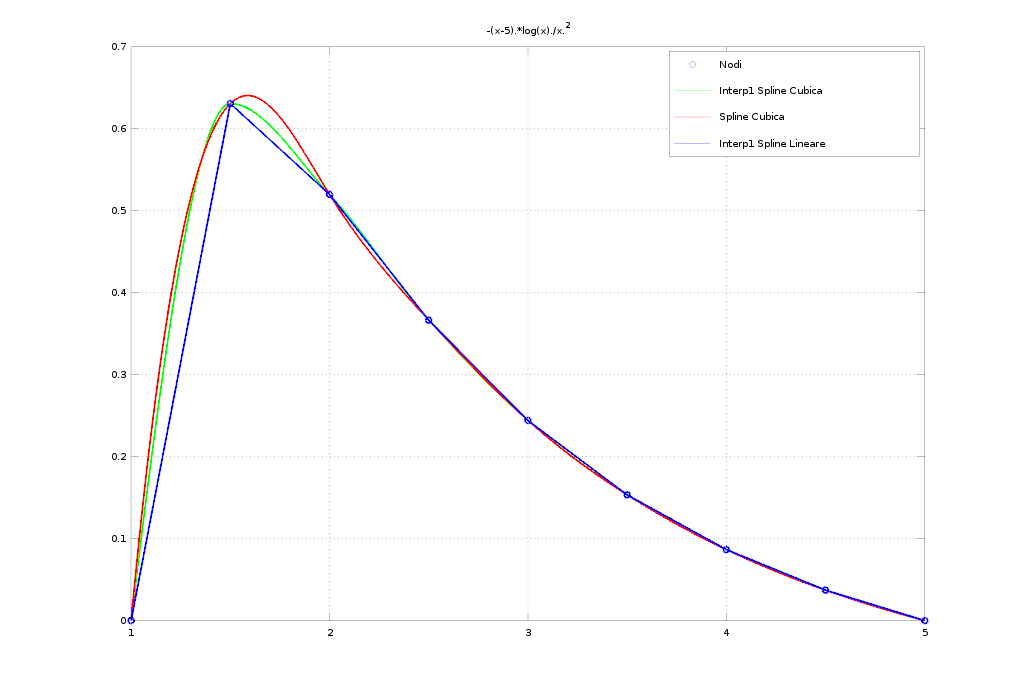
\includegraphics[scale=0.6]{ex62.png}}


%%%%%%%%%%%%%%%%%%%%%%%%%%%%%%%%%%%%%%%%%%%%%%%%%%%%%%%%%%%%%%%%%%%%%%%%%%%%%%%%%%%%%
\newpage
\subsection{ Esercizio 3}
\begin{lstlisting}
load csape.m

x = [-1, -0.5, 0, 0.5, 1];
y = [0.5, 0.8, 1, 0.8, 0.5];
 
xx = linspace(-1,1,1000);

% "Complete" condition imposes that the spline's values  have to be clamped 
%  at the extreme knots with values specified in 2nd argument vector
pp_cl = csape(x,y,'complete',[1/2 -1/2]);

% Not-a-knot condition imposes the continuity of third derivative between first and second and
%   next-to-last and last knot-
pp_nk = csape(x,y,'not-a-knot');

yy_cl = ppval(pp_cl,xx);
yy_nk = ppval(pp_nk,xx);

plot(xx,yy_cl,'linewidth',2,'r',xx,yy_nk,'linewidth',2,'b');
grid on
legend(" Spline Vincolata ", " Not-a-Knot Spline ");

\end{lstlisting}


\centerline{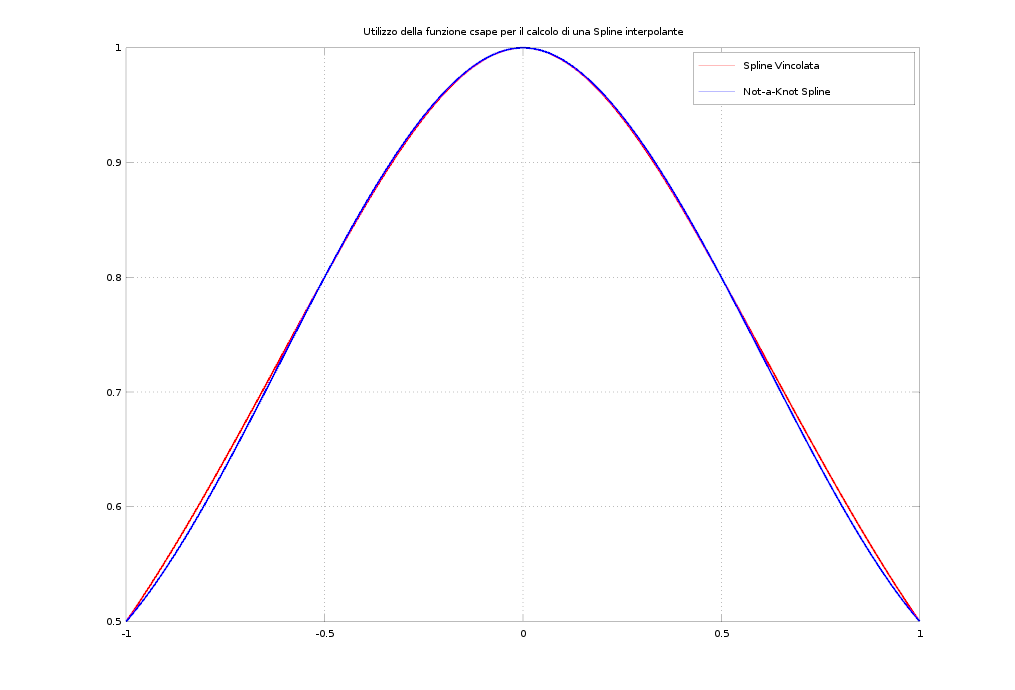
\includegraphics[scale=0.6]{ex63.png}}


%%%%%%%%%%%%%%%%%%%%%%%%%%%%%%%%%%%%%%%%%%%%%%%%%%%%%%%%%%%%%%%%%%%%%%%%%%%%%%%%%%%%%
\newpage
\subsection{ Esercizio 4}
\begin{lstlisting}
load csape.m

x = linspace(0,2*pi,500);
y = sin(x);

xx = linspace(0,2*pi,50);
yy = sin(xx);

% Cofficents Periodic Spline 
%    S'(x0) = S'(xn)
%    S''(x0) = S''(xn)

cp = csape(x,y,'periodic');




% Coefficents Natural Spline 
%    S'''(x0)=S'''(xn) = 0

cn = csape(x,y,'complete',[ 0 0 ]);



yp = ppval(cp,xx);
yn = ppval(cn,xx);

err_periodic = abs(yy-yp);
err_natural  = abs(yy-yn);


subplot(2,1,1)
  plot(x,y,'linewidth',2,'g', xx,yp,'linewidth',0.5,'b', xx,yn,'linewidth',2,'r')
  title(" Interpolazione del seno con spline cubiche naturali e periodiche ");
  grid on
  legend(" sin(x) ", " periodic spline ", " natural spline ");
subplot(2,1,2)
  plot(xx,err_periodic,'linewidth',2,'r', xx,err_natural,'linewidth',2,'b')
  title(" errori interpolatori di spline periodiche e naturali ");
  grid on
  legend( " Errore spline periodica ", " Errore spline naturale ");



% Si noti che data una discretizzazione iniziale piccola ( 5 punti ) come questa
%  gli errori risultano rilevanti per entrambe le tecniche interpolatorie, per quanto per la
%  spline naturale risultino gi\'{a} maggiori.
% Se aumentiamo notevolmente invece il numero di intervalli notiamo che entrambi gli errori
%  tendono a diminuire drasticamente all'interno dell'intervallo, mentre agli estremi la
%  spline naturale continua a mantenere un errore notevole.
\end{lstlisting}



\centerline{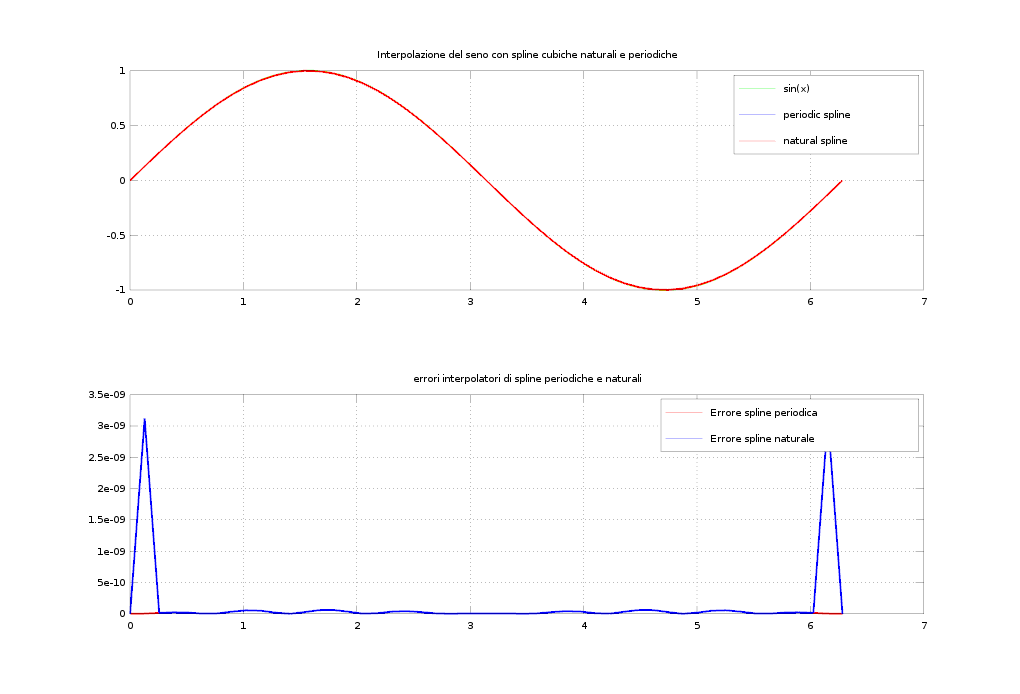
\includegraphics[scale=0.6]{ex64.png}}


%%%%%%%%%%%%%%%%%%%%%%%%%%%%%%%%%%%%%%%%%%%%%%%%%%%%%%%%%%%%%%%%%%%%%%%%%%%%%%%%%%%%%
\newpage
\subsection{ Esercizio 5}
\begin{lstlisting}
p1 = [ 2, -3, 4, -7 ];
p2 = [ 3, -2, -5 ];

% Somma di Polinomi

 psum = polyadd(p1,p2);

% Sottrazione di Polinomi

 psub = polyadd(p1,-p2);

% Moltiplicazione

 pmul = conv(p1,p2);

% Divisione 
 
 pdiv = deconv(p1,p2);


\end{lstlisting}


%%%%%%%%%%%%%%%%%%%%%%%%%%%%%%%%%%%%%%%%%%%%%%%%%%%%%%%%%%%%%%%%%%%%%%%%%%%%%%%%%%%%%
\newpage
\subsection{ Esercizio 6}
\begin{lstlisting}
f = inline(" e.^-x ");

x = linspace(-3,3,9);

y = f(x);

% Polinomio di grado minimo

 cp = polyfit(x,y,8);

 xx = linspace(-3,3,1000);

% Valori del Polinomio
 
 yp = polyval(cp,xx);


% Ricerca dei Nodi di Chebychev


cheb = inline("1/2(-3+3) + 1/2(3+3)*cos((2*x-1)/(2*9))");

  xc = zeros(1,9);
  for i=1:9 
    xc(i) = 1/2*(-3+3)+1/2*(3+3).*(cos(((2.*i-1)./18).*pi));
  endfor 


yc = f(xc);

% Polinomio di grado minimo con
 Chebychev

 cc = polyfit(xc,yc,8);

% Valori del Polinomio di grado minimo 

 ypc = polyval(cc,xx);


% Errori

y_ex = f(xx);
err_pol  = abs(y_ex-yp);
err_cheb = abs(y_ex-ypc);


% Plotting
 
subplot(2,1,1)
  plot(x,y,'linewidth',2,'o',xx,yp,'linewidth',2,'r',xx,ypc,'linewidth',2,'g');
  legend("Nodi", "Interpolazione su nodi semplici", "Interpolazione su nodi di Chebychev");

subplot(2,1,2)
  plot(xx,err_pol,'linewidth',2,'r',xx,err_cheb,'linewidth',2,'g');
  legend("Errori interpolazione nodi semplici","Errore interpolazione nodi di Chebychev");
\end{lstlisting}



\centerline{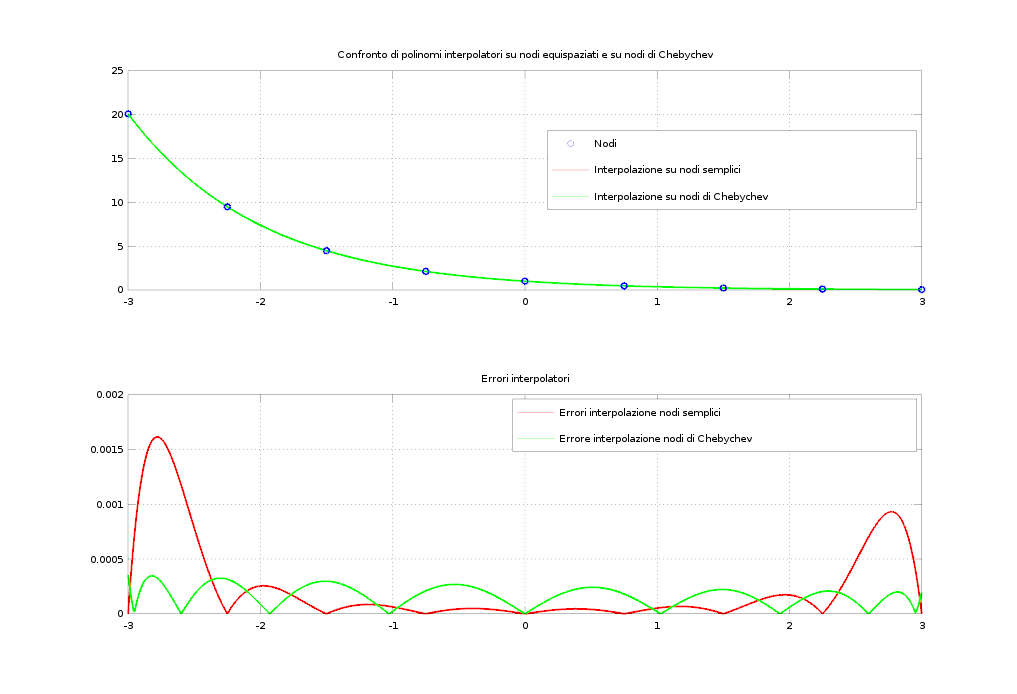
\includegraphics[scale=0.6]{ex66.png}}


%%%%%%%%%%%%%%%%%%%%%%%%%%%%%%%%%%%%%%%%%%%%%%%%%%%%%%%%%%%%%%%%%%%%%%%%%%%%%%%%%%%%%
\newpage
\subsection{ Esercizio 7}
\begin{lstlisting}
f = inline("sin(x) + log(x) -1 ");
x = [1.5, 4, 5, 5.5, 8];
y = f(x);

xx = linspace(1,9,1000);

c = polyfit(x,y,4);

yy = polyval(c,xx);

y_ex = f(xx);


err = abs(y_ex-yy);


subplot(2,1,1)
plot(x,y,'linewidth',3,'o',xx,y_ex,'linewidth',2,'r', xx,yy,'linewidth',2,'b');
legend(" Nodi ", " sin(x) + log(x) -1 ", " Polinomio di 4 grado ","location","northwest");
grid on
ylabel(" sin(x) + log(x) -1 ");

subplot(2,1,2)
plot(xx,err,'linewidth',2,'r');
title(" Errori Interpolatori ")
grid on

\end{lstlisting}


\centerline{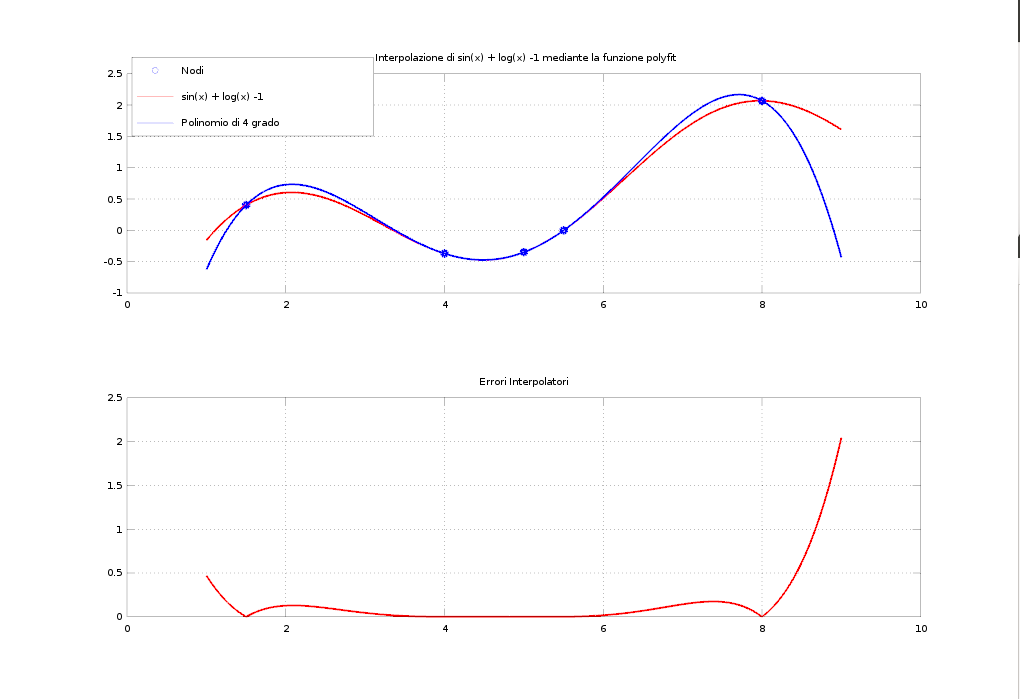
\includegraphics[scale=0.6]{ex67.png}}


%%%%%%%%%%%%%%%%%%%%%%%%%%%%%%%%%%%%%%%%%%%%%%%%%%%%%%%%%%%%%%%%%%%%%%%%%%%%%%%%%%%%%
\newpage
\subsection{ Esercizio 8}
\begin{lstlisting}
f = inline("1./(1+25*x.^2)");

x9 = linspace(-1,1,9);
x10 = linspace(-1,1,10);
x11 = linspace(-1,1,11);
x12 = linspace(-1,1,12);

y9 = f(x9);
y10 = f(x10);
y11 = f(x11);
y12 = f(x12);


c9 = polyfit(x9,y9,8);
c10 = polyfit(x9,y9,9);
c11 = polyfit(x9,y9,10);
c12 = polyfit(x9,y9,11);

xx = linspace(-1,1,1000);

y_ex = f(xx);
yp9 = polyval(c9,xx);
yp10 = polyval(c10,xx);
yp11 = polyval(c11,xx);
yp12 = polyval(c12,xx);


plot(xx,y_ex,'r',xx,yp9,xx,yp10,xx,yp11,xx,yp12);
legend(" Funzione di Runge Esatta ", " Polinomio di 9 grado ", " Polinomio di 10 grado ", " Polinomio di 11 grado ", " Polinomio di 12 grado ","location","south");
grid on
title(" Approssimazione della funzione di Runge mediante polinomi interpolatori di grado 9,10,11,12");
\end{lstlisting}


\centerline{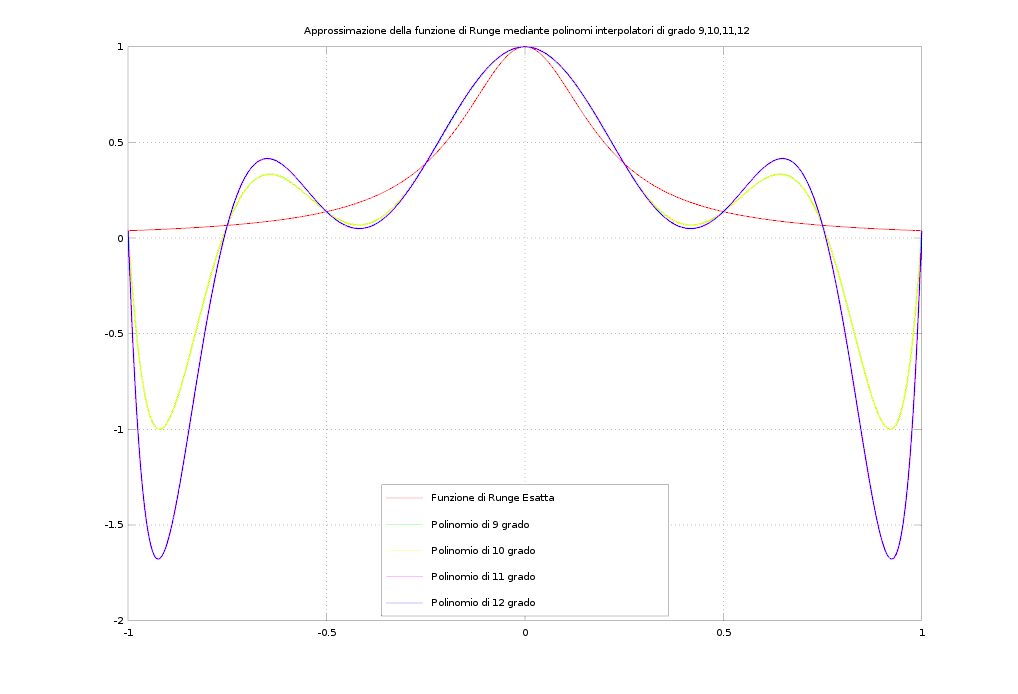
\includegraphics[scale=0.6]{ex68.png}}


%%%%%%%%%%%%%%%%%%%%%%%%%%%%%%%%%%%%%%%%%%%%%%%%%%%%%%%%%%%%%%%%%%%%%%%%%%%%%%%%%%%%%
%%%%%%%%%%%%%%%%%%%%%%%%%%%%%%%%%%%%%%%%%%%%%%%%%%%%%%%%%%%%%%%%%%%%%%%%%%%%%%%%%%%%%
\section{Esercitazione 7}


%%%%%%%%%%%%%%%%%%%%%%%%%%%%%%%%%%%%%%%%%%%%%%%%%%%%%%%%%%%%%%%%%%%%%%%%%%%%%%%%%%%%%
\subsection{Esercizio 1 \\  Costruzione di una formula di quadratura per il calcolo dell' integrale definito $I=\int_{0}^{1} e^{-x^{2}}\,dx$}
\begin{lstlisting}
%% Newton Cotes con n = 4 %%


% expr0= ((x-1)/(0-1))*((x-2)/(0-2))*((x-3)/(0-3))*((x-4)/(0-4));
% expr2= ((x-0)/(2-0))*((x-1)/(2-1))*((x-3)/(2-3))*((x-4)/(2-4));


% Codice per il Calcolo dei Coefficienti in Matlab
syms x;

alpha0 =  int(((x-1)/(0-1))*((x-2)/(0-2))*((x-3)/(0-3))*((x-4)/(0-4))  ,x,  0,  4);

alpha2 =  int(((x-0)/(2-0))*((x-1)/(2-1))*((x-3)/(2-3))*((x-4)/(2-4))  ,x,  0,  4);

alpha1 = (4-(2*alpha0)*-alpha2);
alpha1 = alpha1/2;
alpha3 = alpha1;
alpha4 = alpha0;

#{
% Coefficienti precalcolati
alpha0 = 14/15;
alpha1 = 64/15;
alpha2 = 24/25;
alpha3 = alpha1;
alpha4 = alpha0; 
#}

% alpha0+alpha1+alpha2+alpha3+alpha4 = 4 ? Propriet\'{a} delle costanti di Newton
%  se non vale i calcoli sono errati

alpha = [ alpha0, alpha1, alpha2, alpha3, alpha4 ]


% La formula di NewtonCotes chiusa vuole che I = h*[alpha0*f(x(0)+alpha1*f(x)...]

a=0;
b=1;
h = (b-a)/4;

x = [];
x = [ x, 0 ];
for i=1:4
  x = [ x, a+i*h ];
endfor


f = inline("e^(-x.^2)");
fun = @(x) e^(-x.^2);
y = f(x);

I = 0;
for i=1:5
  I = I + y(i)*alpha(i);
endfor

  I = h*I;

RealI = integrate(fun,0,1);

err = abs(RealI-I);

\end{lstlisting}


%%%%%%%%%%%%%%%%%%%%%%%%%%%%%%%%%%%%%%%%%%%%%%%%%%%%%%%%%%%%%%%%%%%%%%%%%%%%%%%%%%%%%
\newpage
\subsection{Esercizio 2 \\ Costruzione di un grafico per la rappresentazione dell'errore relativo nel calcolo delle formule di Newton-Cotes approssimanti l'integrale definito $I=\int_{0}^{1} e^{-x^{2}}\,dx$}
\begin{lstlisting}
% Andamento dell'errore relativo nel calcolo dell'integrale definito della funzione e^(-x.^2)
%  mediante l'uso delle formule di Newton-Cotes

% Inizio calcolando il valore "esatto" dell'integrale


f = @(x) e.^(-x.^2);


%RealI = integrate(fun,0,1);
%err = abs(RealI-I);

RealI = 0.746824;
RealI_v = RealI*ones(1,7);

% Matrice dei Coefficienti delle formule di Newton-Cotes
NC\_coeff =
\end{lstlisting}


\[
\begin{pmatrix}


                  
      	1/2        &1/2         &0          &0           &0           &0          &0           &0  \\
        1/3        &4/3         &1/3        &0           &0           &0          &0           &0  \\
        3/8        &9/8         &9/8        &3/8         &0           &0          &0           &0  \\
        14/45      &64/45       &24/45      &64/45       &14/45       &0          &0           &0  \\
        95/288     &375/288     &250/288    &250/288     &375/288     &95/288     &0           &0  \\
        41/140     &216/140     &27/140     &272/140     &27/140      &216/140    &41/140      &0  \\
        5257/17208 &25039/17208 &9261/17208 &20923/17208 &20923/17208 &9261/17208 &25039/17208 &5257/17208 

\end{pmatrix}                
\]

\begin{lstlisting}%
[firstnumber=last]
% Ora cerco i 7 valori dell'integrale approssimato

a=0;
b=1;
n=7;

I = zeros(1,n);

for i=1:n
  h = (b-a)/i;
  for j=1:i+1
    I(i) = I(i) + NC_coeff(i,j)*f(a+h*(j-1));
  endfor
  I(i) = h*I(i);
endfor


err = abs(RealI_v - I);

plot([1:7], err, 'linewidth',2,'r')
grid minor
title("Andamento dell'errore di integrazione al crescere della decomposizione \n calcolato come differenza tra RealI = 0.746824 e il valore dato dalla formula per un n dato ");
xlabel("Indice della decomposizione")



% Calcolo ora una stima dell'errore per eccesso mediante le formule alle derivate

f2 = @(x) e.^(-x.^2).*(4*x-2);
f4 = @(x) 4*e.^(-x.^2).*(4*x.^3-2*x.^2-6*x+1);
f6 = @(x) 8*e.^(-x.^2).*(8*x.^5-4*x.^4-40*x.^3+12*x.^2+30*x-3);
f8 = @(x) 16*e.^(-x.^2).*(16*x.^7-8*x.^6-168*x.^5+60*x.^4+420*x.^3-90*x.^2-210*x+15);


a = 0;
b = 1;
h1 = (b-a);
h2 = (b-a)/2;
h3 = (b-a)/3;
h4 = (b-a)/4;
h5 = (b-a)/5;
h6 = (b-a)/6;
h7 = (b-a)/7;


% coefficienti dell'errore
coeff_err  = [ (-1/12)*h1^3, (-1/90)*h2^5, (-3/80)*h3^5, (-8/945)*h4^7, (-275/12096)*h5^7, (-9/1400)*h6^9, (-8183/518400)*h7^9 ];


x = 0:0.01:1;


ve1 = f2(x).*coeff_err(1);
ve2 = f4(x).*coeff_err(2);
ve3 = f4(x).*coeff_err(3);
ve4 = f6(x).*coeff_err(4);
ve5 = f6(x).*coeff_err(5);
ve6 = f8(x).*coeff_err(6);
ve7 = f8(x).*coeff_err(7);

% Cerco il massimo di ogni vettore per poter fare una stima per eccesso

Me1 = max(abs(ve1));
Me2 = max(abs(ve2));
Me3 = max(abs(ve3));
Me4 = max(abs(ve4));
Me5 = max(abs(ve5));
Me6 = max(abs(ve6));
Me7 = max(abs(ve7));


Me=[Me1,Me2,Me3,Me4,Me5,Me6,Me7];



figure 2
plot(1:7,Me,'linewidth',2,'g');
grid minor
title("Andamento dell'errore interpolatorio calcolato al crescere della decomposizione \n calcolato mediante le tabelle degli errori ");

\end{lstlisting}

\centerline{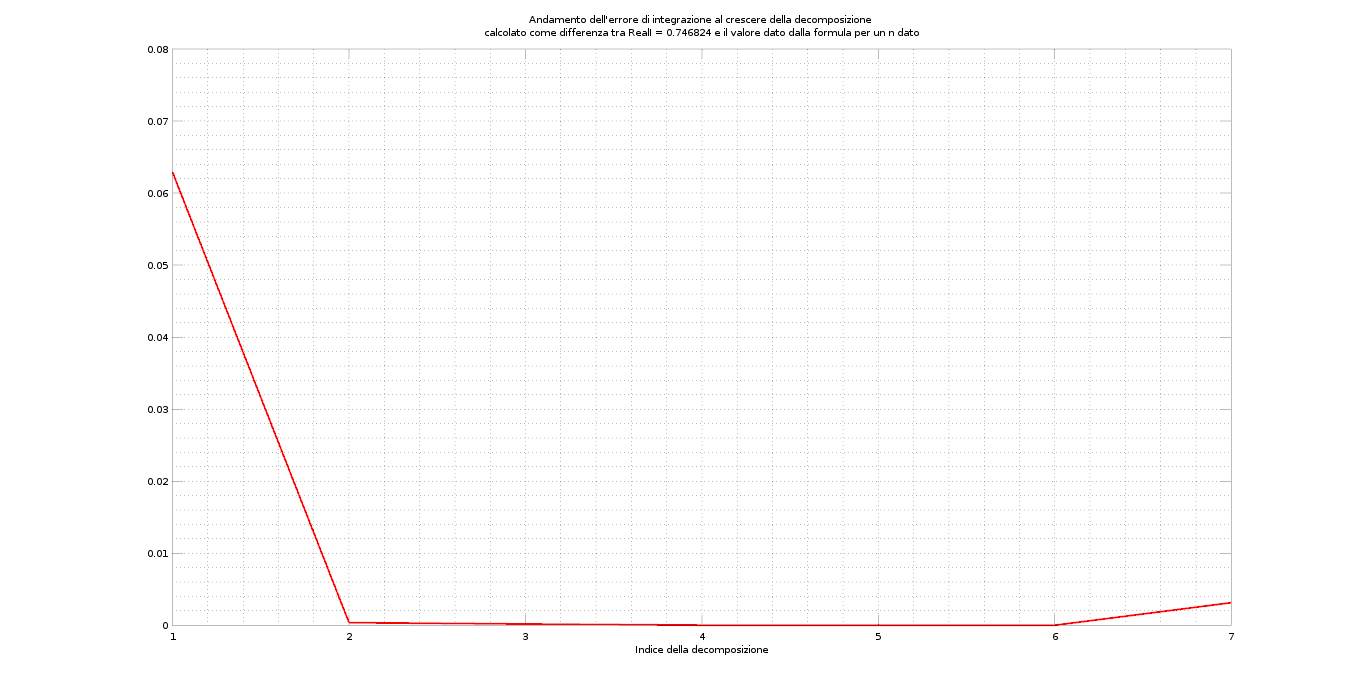
\includegraphics[scale=0.5]{ex72a.png}}
\centerline{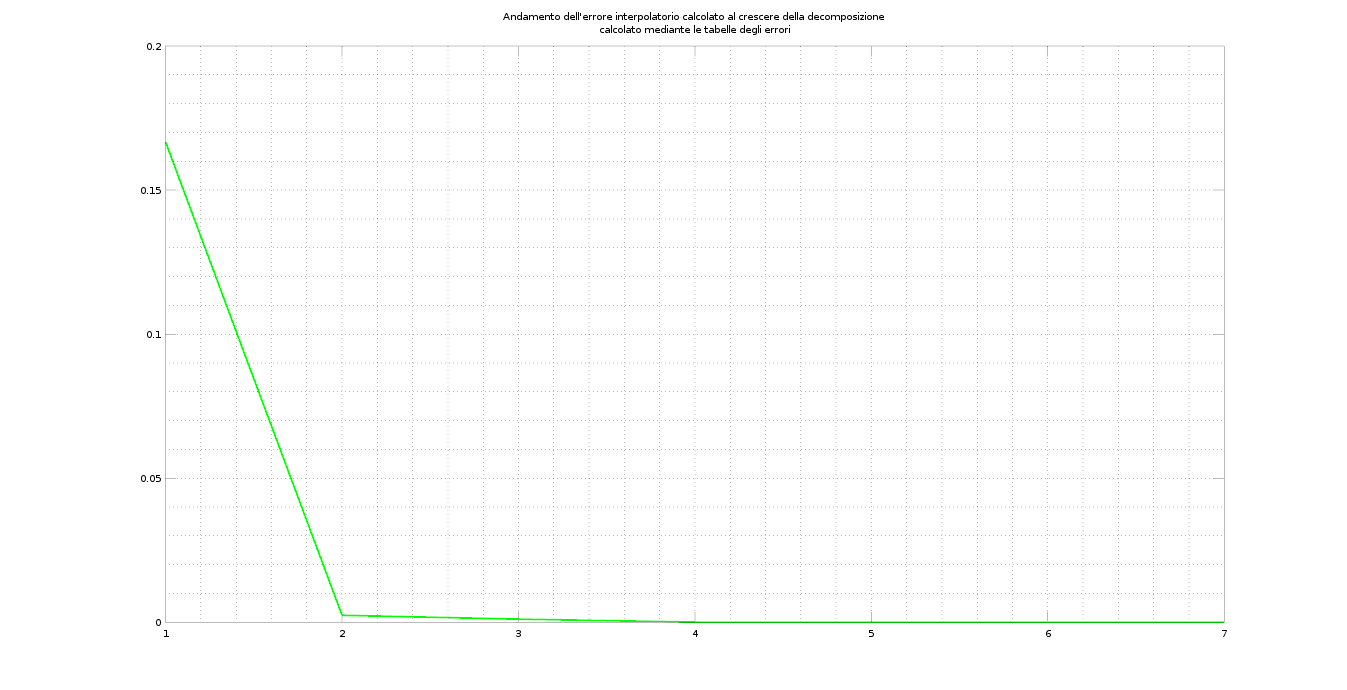
\includegraphics[scale=0.5]{ex72b.png}}

%%%%%%%%%%%%%%%%%%%%%%%%%%%%%%%%%%%%%%%%%%%%%%%%%%%%%%%%%%%%%%%%%%%%%%%%%%%%%%%%%%%%%
\newpage
\subsection{Esercizio 3  \\ Costruzione di un grafico per la rappresentazione degli errori relativi nel calcolo dell'integrale definito $\int_{0}^{1} sin(x)\,dx$ mediante le formule dei trapezi e di Cavalieri-Simpson iterate }
\begin{lstlisting}
% Errori relativi al calcolo dell'integrale definito tra 0 e 1
%  della funzione sin(x) con le formule di Cavalieri Simpson
%  al crescere dei sottointervalli della decomposizione


% RealI = integrate(0,1,@(x) sin(x));
% Calcolato Online risulta
RealI = 0.45970;

CS_coeff = [ 1/3, 4/3, 1/3 ];

b0 = 1;
a0 = 0;

b = @(i,j) a0 + j*((b0-a0)/i),
a = @(i,j) (j-1)/i;

% Voglio dividere l'intervallo in 2m sottointervalli di modo da poter 
%  applicare la formula di CavalieriSimpson sottointervalli sulle coppie di sottointervalli
% Lo far\'{o} per n=1:10

 
function I = CavalieriSimpson(x,y,f)
   I = ((y-x)/2)*(1/3*f(x) + 4/3*f((x+y)/2) + 1/3*f(y));
endfunction

I = zeros(10);

for i=1:10
  for j=1:i
    I(i,j) = CavalieriSimpson(a(i,j),b(i,j),@(x) sin(x));
  endfor
endfor



% sommando i termini della stessa riga della matrice I ottengo un'approssimazione ( in teoria sempre migliore )
%  del valore dell'integrale del seno di x tra 0 e 1


Integralen = zeros(1,10);

for i=1:10
  for j=1:i
    Integralen(i) = Integralen(i) + I(i,j);
  endfor
endfor


RealIv = ones(1,10)*RealI;

err_rel = abs(RealIv-Integralen)./RealIv;

plot([1:10],err_rel,'linewidth',2,'r');
title(" Andamento degli errori relativi al crescere del valore della decomposizione ");
grid minor

\end{lstlisting}

\centerline{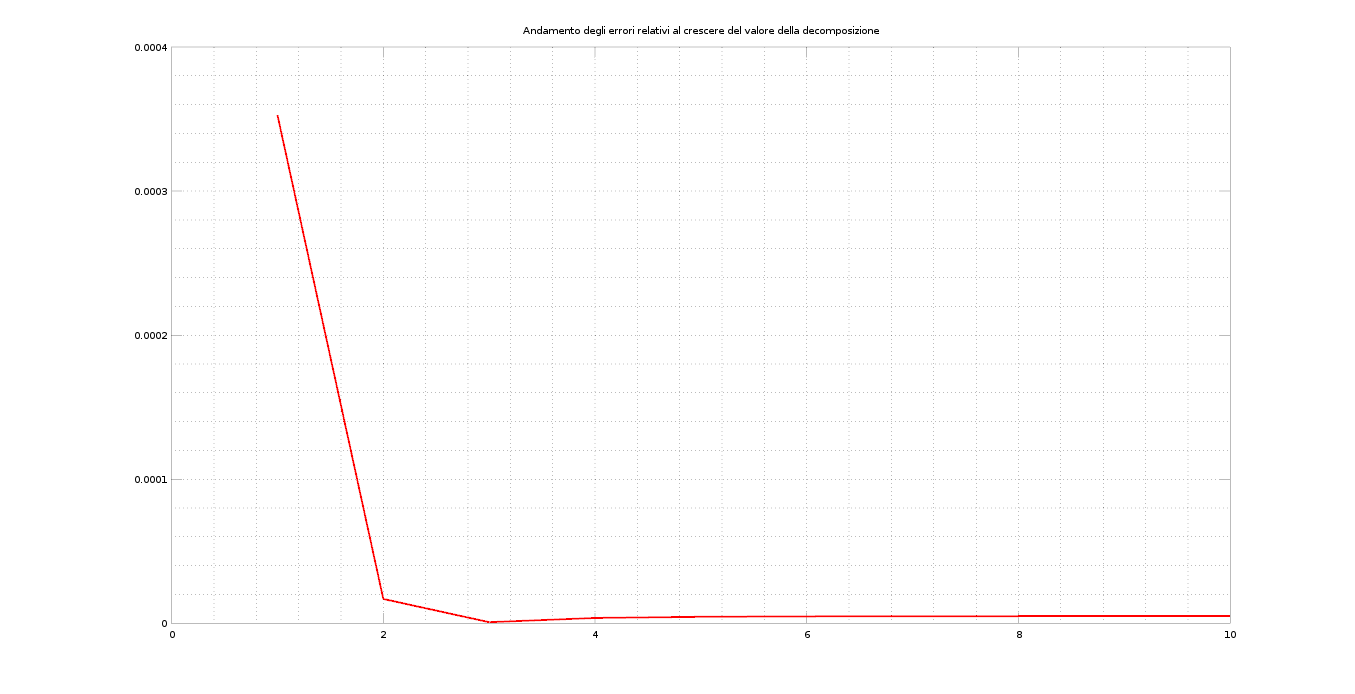
\includegraphics[scale=0.5]{ex73.png}}


%%%%%%%%%%%%%%%%%%%%%%%%%%%%%%%%%%%%%%%%%%%%%%%%%%%%%%%%%%%%%%%%%%%%%%%%%%%%%%%%%%%%%
%%%%%%%%%%%%%%%%%%%%%%%%%%%%%%%%%%%%%%%%%%%%%%%%%%%%%%%%%%%%%%%%%%%%%%%%%%%%%%%%%%%%%
\newpage
\section{ Esercitazione 8}


%%%%%%%%%%%%%%%%%%%%%%%%%%%%%%%%%%%%%%%%%%%%%%%%%%%%%%%%%%%%%%%%%%%%%%%%%%%%%%%%%%%%%
\subsection{Esercizio 1 \\ Utilizzo della tecnica del pivoting per la fattorizzazione LU}
\begin{lstlisting}
function [A, P] = pivoting(A)
    P = eye(length(A));
    for i = 1: length(A)
        if(A(i, i) == 0)
            [m, j] = max(abs(A(i:length(A), i)));
            j = i + j - 1;
            A([i,j],:) = A([j,i],:);
            P([i,j],:) = P([j,i],:);
        end
    end
end


% fattorizzazione LU

function [ L, U, P ] = lu_fact(A)
   [ A, P ] = pivoting(A);
   n = size(A);
   L = eye(n);
   U = zeros(n);

   for k=1:n-1
     for i=k+1:n
       L(i,k) = A(i,k)/A(k,k);
       A(i,:) = A(i,:) - L(i,k)*A(k,:);
     endfor
   endfor

   U = A;
endfunction



A1 =
       1, 0, 0, 1; 
       1, 0, 0, 1; 
       0, 0, 1, 1;
       2, 3, 4, 5; 

A2 =
       4, 0,  2,  4; 
       0, 1,  1,  1;
       2, 2, 11   9; 
       4, 1,  9, 25; 	
\end{lstlisting}

\newpage

\begin{lstlisting}%
[firstnumber=last]
[ l1, u1, p1 ] = lu_fact(A1);

[ l2, u2, p2 ] = lu_fact(A2);


[ ll1, uu1, pp1 ] = lu(A1);
[ ll2, uu2, pp2 ] = lu(A2);

% Fattorizzazione con lu_fact di A1
l1 =

   1   0   0   0
   2   1   0   0
   0   0   1   0
   1   0   0   1

u1 =

   1   0   0   1
   0   3   4   3
   0   0   1   1
   0   0   0   0

p1 =

   1   0   0   0
   0   0   0   1
   0   0   1   0
   0   1   0   0

p1*(l1*u1) =

   1   0   0   1
   1   0   0   1
   0   0   1   1
   2   3   4   5

A1 =

   1   0   0   1
   1   0   0   1
   0   0   1   1
   2   3   4   5


% Fattorizzazione con lu_fact di A2

l2 =

   1.00000   0.00000   0.00000   0.00000
   0.00000   1.00000   0.00000   0.00000
   0.50000   2.00000   1.00000   0.00000
   1.00000   1.00000   0.75000   1.00000

u2 =

    4.00000    0.00000    2.00000    4.00000
    0.00000    1.00000    1.00000    1.00000
    0.00000    0.00000    8.00000    5.00000
    0.00000    0.00000    0.00000   16.25000

p2 =

% Essendo la matrice di permutazione diagonale si pu\'{o} dedurre che nessuno dei minori
%  di A2 abbia determinante nullo, quindi non necessita di una premoltiplicazione per una
%  matrice di permutazione.

Diagonal Matrix

   1   0   0   0
   0   1   0   0
   0   0   1   0
   0   0   0   1

p2*(l2*u2) =

    4    0    2    4
    0    1    1    1
    2    2   11    9
    4    1    9   25



A2 =

    4    0    2    4
    0    1    1    1
    2    2   11    9
    4    1    9   25



% Fattorizzazione con lu di matlab di A1
ll1 =

   1.00000   0.00000   0.00000   0.00000
   0.50000   1.00000   0.00000   0.00000
   0.00000  -0.00000   1.00000   0.00000
   0.50000   1.00000   0.00000   1.00000

uu1 =

   2.00000   3.00000   4.00000   5.00000
   0.00000  -1.50000  -2.00000  -1.50000
   0.00000   0.00000   1.00000   1.00000
   0.00000   0.00000   0.00000   0.00000

pp1 =

Permutation Matrix

   0   0   0   1
   0   1   0   0
   0   0   1   0
   1   0   0   0
 \end{lstlisting}

\newpage

\begin{lstlisting}%
[firstnumber=last]
pp1*(ll1*uu1) =

   1   0   0   1
   1   0   0   1
   0   0   1   1
   2   3   4   5

A1 =

   1   0   0   1
   1   0   0   1
   0   0   1   1
   2   3   4   5


% Fattorizzazione con lu di matlab di A2

ll2 =

   1.00000   0.00000   0.00000   0.00000
   0.50000   1.00000   0.00000   0.00000
   0.00000   0.50000   1.00000   0.00000
   1.00000   0.50000  -0.50000   1.00000

uu2 =

    4.00000    0.00000    2.00000    4.00000
    0.00000    2.00000   10.00000    7.00000
    0.00000    0.00000   -4.00000   -2.50000
    0.00000    0.00000    0.00000   16.25000
\end{lstlisting}

\newpage

\begin{lstlisting}%
[firstnumber=last]
pp2 =
Permutation Matrix

   1   0   0   0
   0   0   1   0
   0   1   0   0
   0   0   0   1

 octave:172> pp2*(ll2*uu2)
ans =

    4    0    2    4
    0    1    1    1
    2    2   11    9
    4    1    9   25

A2 =

    4    0    2    4
    0    1    1    1
    2    2   11    9
    4    1    9   25


%Le matrici di permutazione restituite dall'algoritmo implementato nel
% linguaggio non sono le stesse che ottengo dal mio algoritmo.
% Evidentemente l'implementazione interna utilizza un algoritmo differente
% da quello di eliminazione gaussiana.



\end{lstlisting}

%%%%%%%%%%%%%%%%%%%%%%%%%%%%%%%%%%%%%%%%%%%%%%%%%%%%%%%%%%%%%%%%%%%%%%%%%%%%%%%%%%%%%
\newpage
\subsection{Esercizio 2 \\ Implementazione dei metodi di Jacobi e di Gauss-Seidel per la soluzione approssimata di sistemi lineari1}

\begin{lstlisting}
A1 
       -3, 3, -6 
       -4, 7, -8 
        5, 7, -9

b1 = -6; -5; 3 


A2 = 
        4,  1,  1
        2, -9,  0
        0, -8, -6

b2 = 6; -7; -14 


function [ xnew, err, ro ] = Jacobi(A,b,x0,Nmax,toll)

  D = diag(A);
  E = D-tril(A);
  F = D-triu(A);

  invD = diag(1./diag(A));
  Pj = invD*(E+F);  % Matrice di iterazione
  ro = max(abs(eig(Pj)));  

  xold = x0;
  i=1;
  test = 1;
  err = zeros(1,Nmax);
  
  while i<Nmax && test>toll
    xnew   = Pj*xold + invD*b;   % Da definizione
    err(i) = norm(xnew-xold);
    test   = err(i);
    xold   = xnew;
    i      = i+1;
  endwhile

  err = err(1:i-1);

endfunction



function [ xnew, err, ro ] = GaussSeidel(A,b,x0,Nmax,toll)

  D = diag(A);
  E = D-tril(A);
  F = D-triu(A);

  invDE = inv(D+E);
  Pgs = invDE*F;  % Matrice di iterazione
  ro = max(abs(eig(Pgs)));

  xold = x0;
  i=1;
  test = 1;
  err = zeros(1,Nmax);
  
  while i<Nmax && test>toll
    xnew   = Pgs*xold + invDE*b;   % Da definizione
    err(i) = norm(xnew-xold);
    test   = err(i);
    xold   = xnew;
    i      = i+1;
  endwhile

  err = err(1:i-1);

endfunction




[x1j, err1j, ro1j]= Jacobi(A1, b1, zeros(3, 1), 100, 10^-3);
[x2j, err2j, ro2j]= Jacobi(A2, b2, zeros(3, 1), 100, 10^-3);

 
[x1g, err1g, ro1g]= GaussSeidel(A1, b1, zeros(3, 1), 100, 10^-3);
[x2g, err2g, ro2g]= GaussSeidel(A2, b2, zeros(3, 1), 100, 10^-3);



hold on
subplot(2,2,1)
semilogy(1:length(err1j), err1j)
title([ "Jacobi(A1x1=b1), ro(P1j) = " num2str(ro1j) ] )
grid on
subplot(2,2,2)
semilogy(1:length(err2j), err2j)
title([ "Jacobi(A2x2=b2), ro(P2j) = " num2str(ro2j) ] )
grid on
subplot(2,2,3)
semilogy(1:length(err1g), err1g)
title([ "GaussSidel(A1x1=b1), ro(P1g) = " num2str(ro1g) ] )
grid on
subplot(2,2,4)
semilogy(1:length(err2g), err2g)
title(["GaussSidel(A2x2=b2), ro(P2g) = " num2str(ro2g) ])
grid on

[firstnumber=last]
%%% fprintf degli errori %%%%%

e1j = [ 1:length(err1j); err1j ]; 
e2j = [ 1:length(err2j); err2j ]; 

e1g = [ 1:length(err1g); err1g ]; 
e2g = [ 1:length(err2g); err2g ]; 


file_errori = fopen('errori1j.txt','w');
fprintf(file_errori, '%6s %56s\n', 'x', 'errore sistema 1 con Jacobi')
fprintf(file_errori, '%6.2f %56.8f\n' , e1j);

file_errori = fopen('errori2j.txt','w');
fprintf(file_errori, '%6s %56s\n', 'x', 'errore sistema 2 con Jacobi')
fprintf(file_errori, '%6.2f %56.8f\n' , e2j);

file_errori = fopen('errori1g.txt','w');
fprintf(file_errori, '%6s %56s\n', 'x', 'errore sistema 1 con Gauss Sidel')
fprintf(file_errori, '%6.2f %56.8f\n' , e1g);

file_errori = fopen('errori2g.txt','w');
fprintf(file_errori, '%6s %56s\n', 'x', 'errore sistema 2 con Gauss Sidel')
fprintf(file_errori, '%6.2f %56.8f\n' , e2g);


\end{lstlisting}

\centerline{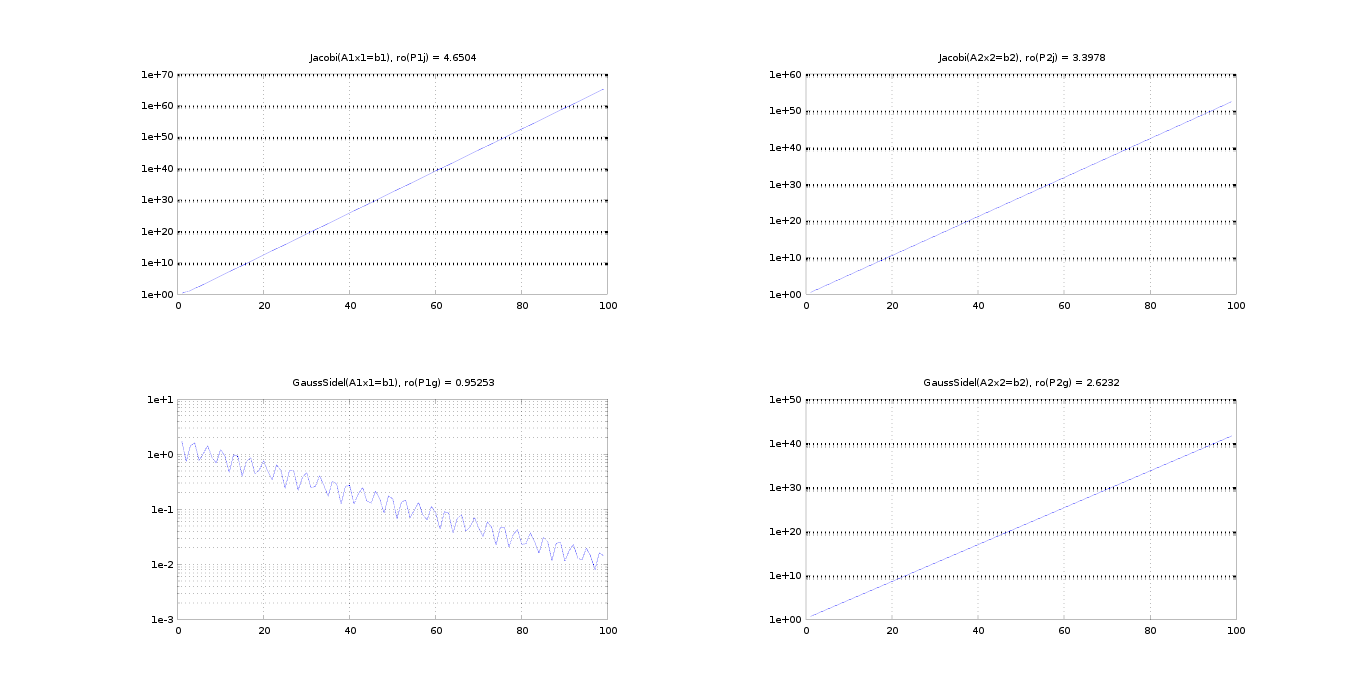
\includegraphics[scale=0.5]{ex82.png}}


\vs
\begin{flushleft}
Si noti che l'unica successione convergente è quella che usa il metodo di Gauss Sidel sul primo dei sistemi, 
la matrice d'iterazione associata infatti ha raggio spettrale minore di 1.\\
Abbiamo un teorema che ci dice che questa è una condizione necessaria e sufficiente, quindi è coerente con la teoria avere come unica successione convergente quella che ha matrice associata d'iterazione con raggio spettrale minore di 1
\end{flushleft}
\vs

\end{document}


